%%----------Chapter 2------------------------------------------
\documentclass[../UNBThesis2.tex]{subfiles}
\setlength{\parindent}{2em}
\begin{document}
\chapter{Background}

As the number of connected devices and applications that generate huge amount of data at very high speed increases, the need for faster datamining techniques is enhanced. This research work proposes a data stream clustering algorithm that builds upon the Affinity Propagation clustering algorithm. The concept of time windows that partition the data into manageable chunks is introduced in order to apply these algorithms for data stream clustering.

This Chapter presents an overview of the clustering and data stream algorithms by reviewing their concepts and underlying mathematics. Furthermore, all the time window models applicable for data stream clustering are introduced. K-means algorithm based clustering techniques are introduced to compare with the proposed model to evaluate it's performance. Real world indoor localization data that is discussed later in the chapter is used to test the model. 


\section{Cluster Analysis}

Clustering refers to partitioning a set of observations or tuples into groups according to some desired criterion \cite{jain1999data}. The intra-cluster objects within a group are similar while the inter-cluster objects are dissimilar. Figure \ref{clus} illustrates the clustering process graphically for a set of points in 2D space that are clustered into three clusters. Each cluster is generally represented by its center or exemplar or centroid of the cluster.

\begin{figure}[!h]
    \centering
    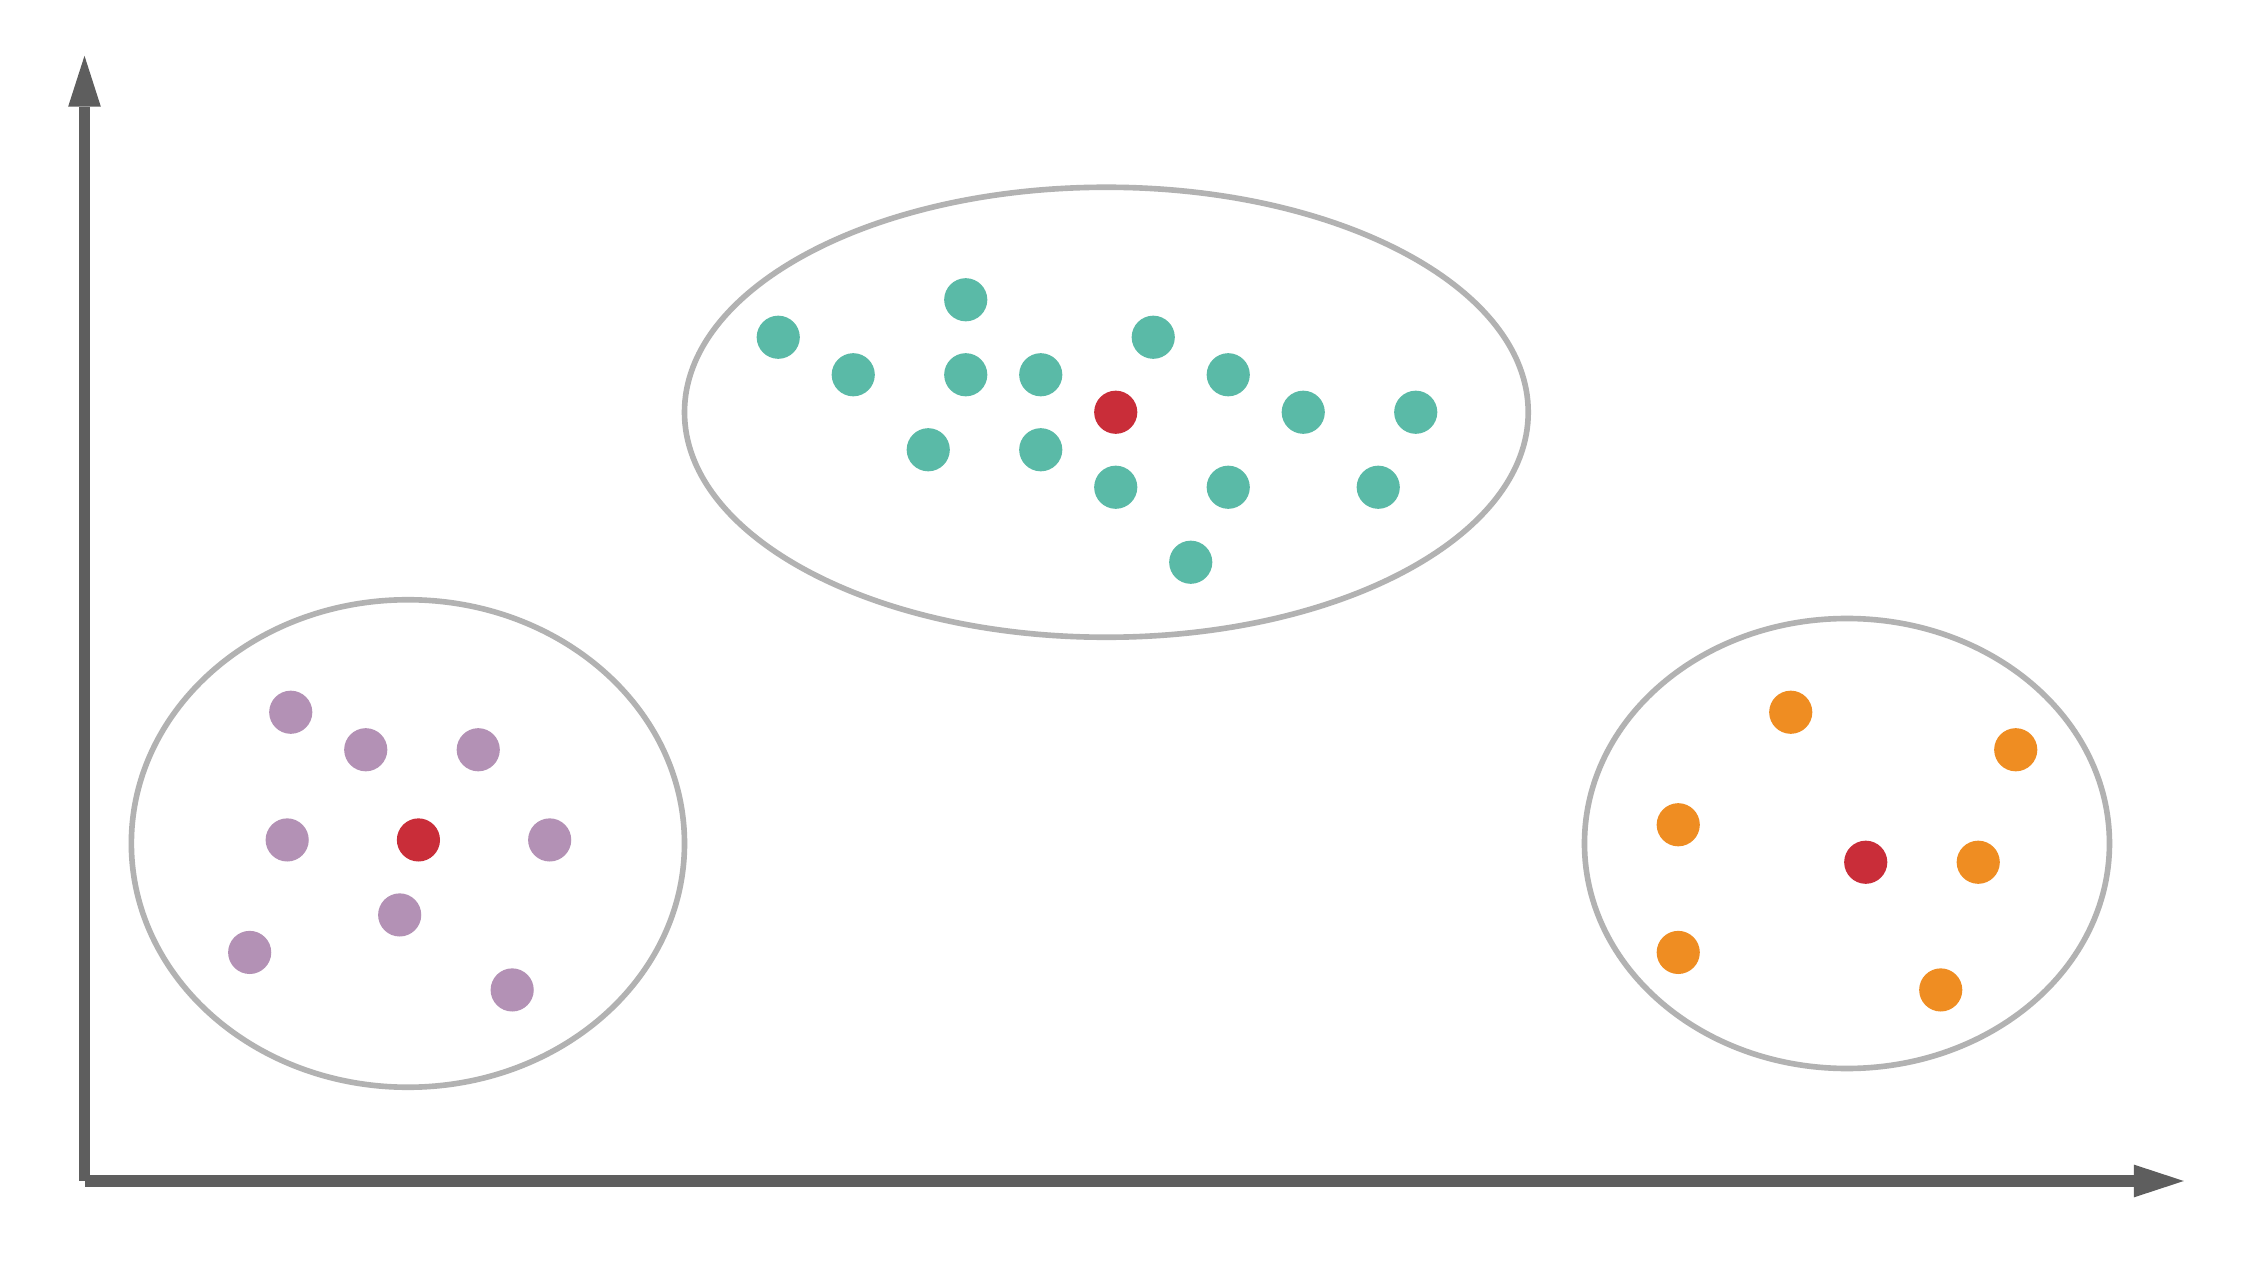
\includegraphics[width = 10 cm]{image/Chapters/Chapter2/Blank diagram (1).png}
    \caption{Data clustering in 2D space. Each of these three clusters has centroid which is shown by the red circle. }
    \label{clus}
\end{figure}


Even though labeled data can be analyzed using clustering techniques, but the strength of this unsupervised approach (or exploratory learning) lies in detecting similarities within an unlabelled dataset. Cluster analysis is used in diverse fields with different goals and applications, such as: 

\begin{enumerate}
    \item Group discovery, which is grouping similar objects into clusters, finding the data distribution, and defining a preliminary stage for discriminant analysis. 
    \item Pattern recognition, is an automated way of finding patterns and regularities in the data by matching the information stored in the database with the incoming data. 
    \item data compression, provides a summary of a dataset by representing its most representative object which can be a center of mass or an actual data point as a centroid.
    \item Outlier detection is another method in which many applications employ anomaly detection, such as intrusion detection, fraud detection. Anomaly detection is achieved by identifying outliers. An outlier can be a data point very far from it's cluster centers or form small clusters that deviate from the prominent clusters.
    \item Feature selection is used when the number of features in the dataset is larger than the number of data points, then dimension reduction or feature selection is necessary to be applied.
\end{enumerate}


Distance (dissimilarity) and similarity between data points are the basis of clustering algorithms \cite{zumel2014practical}. The most commonly used distance functions for quantitative data features are summarized in Table \ref{tabdis}

% and these two words bring distances of each data point in the cluster which is closer to other data points than other data points in other clusters \cite{zumel2014practical}. 


% The Euclidean distance is the most common one, and this is what we applied in our work. It calculated the root of square differences between two pairs of data points.
% Manhattan distance which computes the absolute differences between two data points.
% Minkowski distance is ---
% Cosine distance is a common similarity metric in text analysis. It measures the smallest
% angle between two vectors \cite{zumel2014practical}.
% Mahalanobis distance---
% Categorical data usually applies Hamming distance which a number of attributes taking different values \cite{han2001data}.


\begin{table}[!h]{}
\centering
\caption{Distance metrics for data clustering \protect\cite{xu2015comprehensive}.}
    \label{tabdis}
    \begin{tabular}{p{4cm} l p{5cm} l  p{6cm} }
    \hline
    \textbf{Distance} & \textbf{Formula} & \textbf{Description} \\ \hline
    \midrule
    
    
    
     Euclidean distance             &  
     
    $\sqrt {\sum _{i=1}^{n}  \left( q_{i}-p_{i}\right)^2 }$
%  \left( \sum_{i=1}^k \abs{\frac {q_i - p_i}{s}}^2 \right)
     
  
     &  
     Root square differences between co-ordinates of a pair of objects
     
     \\ \hline
    Minkowski distance                &    
     
 $\left( \sum_{i=1}^n \abs{q_i - p_i}^n \right)^{\frac{1}{n}}$

     
     &  
      1-Euclidean distance if n=2, 2-City-block distance if n=1, 3-Chebyshev distance if n $\leftarrow \infty$
     
     \\
    \hline
    
     Manhattan distance                 &    
     
    $ \sum_{i=1}^n \abs{q_i - p_i}$
     
     
     &  
     in n-dimensional space is the sum of the distances in each dimension
     \\
    \hline
    
    Cosine distance                    &   
    
    $1 - cos \alpha = \frac{q_i^{T} - p_i}{\|q_i\| \|p_i\|}$
   
    
    &  
    1-Stays the same in the face of rotational change in data, 
    2-The most commonly used distance in document area
    \\
    \hline
    
    Mahalanobis distance               &   
    
     
    $\sqrt{(q_i - p_i)^T S^{-1} (q_i - p_i)}$

    &  
    1- S is the co-variance matrix inside the cluster,  
    2- High computation complexity
    \\
    \hline
    \bottomrule

\end{tabular}
\end{table}





There are many data clustering algorithms available for different applications. Selecting an algorithm is important, as certain algorithms are better suited particular datasets and reflect the true nature of the data \cite{berkhin2006survey, han2011data}. Traditionally clustering algorithms are divided into five main types as listed below. The advantages and disadvantages of all these methods are listed next in \ref{methoda}.
%In progress

\begin{itemize}

    \item\textbf{Partitioning methods:} Data is being split into $k$ number of clusters based on the similarities or distances to the cluster centroids. Each data point belongs to one cluster, and each cluster contains at least one data point. These algorithms usually threshold the distance of new data points to the existing micro-clusters, and maybe it comes(happen) a new cluster. These types of algorithms are finding clusters with spherical shapes, and the noise can influence the results. A very famous algorithm in this group is K-means.
    
    \item\textbf{Hierarchical methods:} seeks to build a tree based hierarchical structure from asset of unlabeled data \cite{swarndeep2016overview}. This grouping process is represented in the form of dendrogram. It can be analyzed with the help of statistical method. BIRCH is the algorithm related to this group.
    %elmi
    \item\textbf{Density-based methods:} continue to grow the given cluster as long as the density in the neighborhood. This algorithm is suitable for handling noise in the data. DBSCAN and OPTICS are two famous algorithms in this group. 
exceeds certain threshold
    %elmi
    \item\textbf{Grid-based methods:} are a special category of density-based algorithms, where the regions consists of the grid cells. In particular, the data space is partitioned into a finite number of cells that form a grid structure on which clustering is performed. STING is one of the highly scalable algorithm in this group with the ability to decompose the data set into various levels of detail. 
    %elmi
    \item\textbf{Model-based methods:} try to fit a model to the data, assuming that data are generated from k probability distributions (typically Gaussian).
\end{itemize}




\begin{table}[!h]\scriptsize
% \centering
\caption{ Advantages and disadvantages of clustering methods \protect\cite{mousavi2015data}.}
\label{methoda}  
\small
\begin{tabularx}{\linewidth}{p{3cm} p{5.5cm} p{5.5cm}}
\hline
 \multicolumn{1}{c}{\textit{\textbf{Methods}}} &
 \multicolumn{1}{c}{\textit{\textbf{Advantages}}}   &   
\multicolumn{1}{c}{\textit{\textbf{Disadvantages}}} 
\tabularnewline \hline
\vfill 
 Partitioning    & 
 \begin{enumerate}[*,topsep=0pt,leftmargin=0.2cm]
 \item Easy to implement  
 \item iterative algorithms
\end{enumerate}
\tabitem
&       
\begin{itemize}[*,nosep,leftmargin=0.2cm]
    \setlength\itemsep{0em}
     \item usually pre-defined value for number of clusters  
     \item spherical shaped
\end{itemize} 
\tabularnewline \hline

\vfill
Hierarchical
& 
\begin{itemize}[*,nosep,leftmargin=0.2cm]
    \item Easy to handle any forms of distance   
\end{itemize}
 &       
\begin{itemize}[*,nosep,leftmargin=0.2cm]
    \item Ambiguity of termination criteria 
    \item High complexity
\end{itemize}
\tabularnewline \hline
\vfill
Grid-based
& 
\begin{itemize}[*,nosep,leftmargin=0.2cm]
    \item Fast processing time 
    \item Can handle noise
\end{itemize}
&      

\begin{itemize}[*,nosep,leftmargin=0.2cm]
    \item Higher value for convex clusters like DBSCAN
    \item Limits distance metric to Euclidean
\end{itemize}
\tabularnewline \hline
\vfill
 \textbf{Density-Based}
& 
\begin{itemize}[*,nosep,leftmargin=0.2cm]
    \item Fast to compute
    \item Easy to interpret %as it gives higher value when clusters are dense
\end{itemize}
 &       
\begin{itemize}[*,nosep,leftmargin=0.2cm]
    \item Higher value for convex clusters% compared with density based clusters
\end{itemize}
\tabularnewline \hline
\vfill
 Model-Based
& 
\begin{itemize}[*,nosep,leftmargin=0.2cm]
    \item Specifying the number of clusters automatically based on standard statistics 
    \item Can handle noises            
\end{itemize}
 &       
\begin{itemize}[*,nosep,leftmargin=0.2cm]
    \item Depending on the hypothesized model or structure
\end{itemize} 
\tabularnewline \hline
\vfill
\end{tabularx}
\end{table}





This work is built based on the two very famous partitioning algorithms, affinity propagation and K-means. The detail of these two algorithm are explained in detail.


\subsection{Affinity Propagation Clustering Algorithm}

% $O(N^2logN)$ where N is the number of data points. It can be imagined that if the number of data points is very huge, then it is impossible to do clustering using AP
Affinity propagation (AP) is a partitioning-based clustering algorithm that has been introduced by Frey and Dueck in 2007 \cite{frey2006mixture}. AP works based on the message passing method to find the best representative of clusters which calls centroid or exemplar \cite{jiang2019exemplar, frey2007clustering}. It means to find data points with the maximum similarity to others. The advantage of AP to compare with many clustering algorithms is that this Algorithm does not require the number of clusters as an input, and it makes it unique between many clustering algorithms.


AP considers all data points as a potential exemplar until a good set of clusters with centroids are found. Figure \ref{APPi} shows the gradually emerging of clusters and centroids, but the tenth iterations show the uncertainly of having clusters shows with the faded blue lines until the last and final iteration to find a good cluster solution.

\begin{figure}
\centering
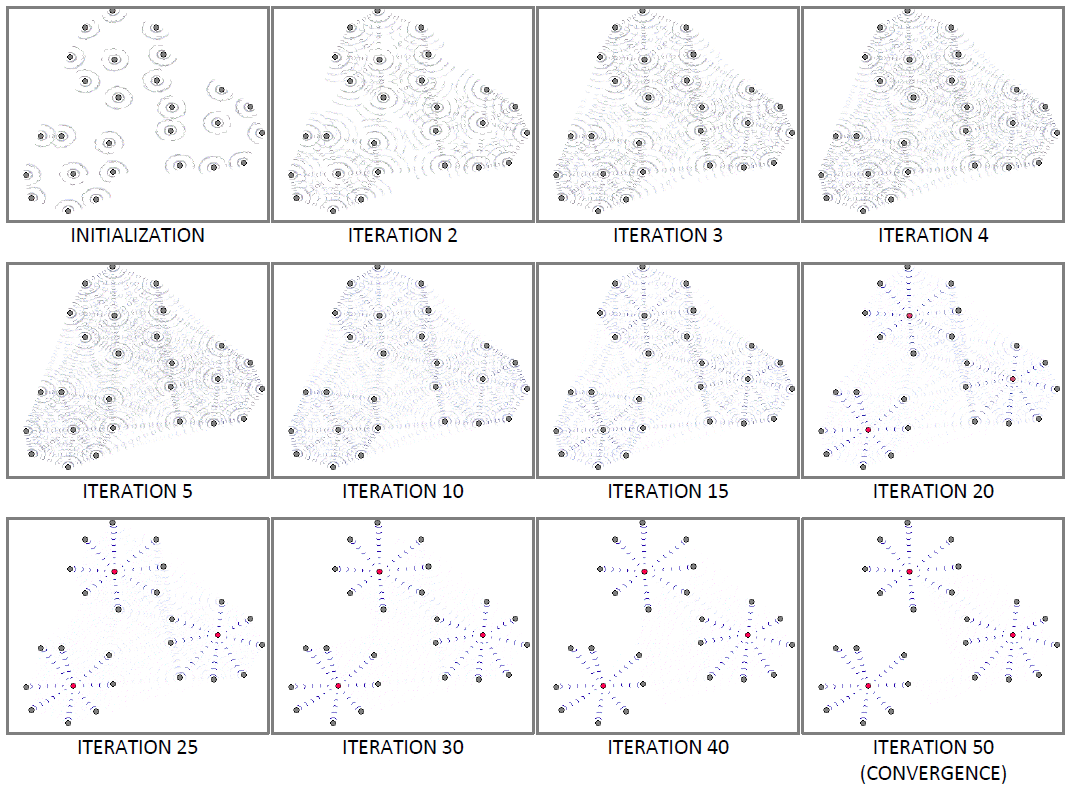
\includegraphics[width = 13 cm]{image/Chapters/Chapter2/APDurek.PNG}
\caption{Affinity propagation: clustering data by passing messages \protect\cite{dueck2009affinity}. It shows the iteration to reach the clusters emerging.}
\label{APPi}
\end{figure}


The AP algorithm consists of four matrices: similarity matrix, responsibility matrix, availability matrix, and Criterion matrix.

\begin{itemize}

  \item\textbf{Similarity matrix:}
  The similarity matrix $s(i,j)$, gives information about any inputs. It shows data points with index \textit{k} is how appropriate to be the cluster-head for data point \textit{i}. Every cell has values that correspond to how similar two objects are. It is a diffident method to calculate the values for diagonal values and non-diagonal values.  The diagonal values,  Cells are filled with the lowest number among all the cells. The non-diagonal values are the negation of the sum of the squares of the differences between participants.
  \item\textbf{Responsibility matrix:} Cells contain values that correspond to how responsible one object is for another. It is better to say how responsible it is to be a part of another object or related to another object. This is calculated with the following equation as shown below:

    \begin{equation}
        r(i, k) \leftarrow s(i, k) - \max\limits_{k' s.t. k' \neq k}\{ a(i, k') + s(i, k') \}
    \end{equation}
    
    
  \item\textbf{Availability matrix:} This matrix contains values that correspond to how available one object is to be an exemplar for another object. With this means, how available one object is for a cluster to be a centroid of a cluster, and diagonal values is the sum of all positive responsibility values in the column excluding the object self-responsibility. 
  The availability diagonal values are determined by the following formulas:

    \begin{equation}
        (i, k) \leftarrow \min\{0, r(k,k) + \sum\limits_{i' s.t. i' \notin \{i, k\}}{\max\{0, r(i', k)\}}
    \end{equation} 
    
    For points on the non-diagonal we have:
    \begin{equation}
        a(k, k) \leftarrow \sum\limits_{i' \neq k}\max(0, r(i', k))
    \end{equation}



    \begin{figure}
    \centering
    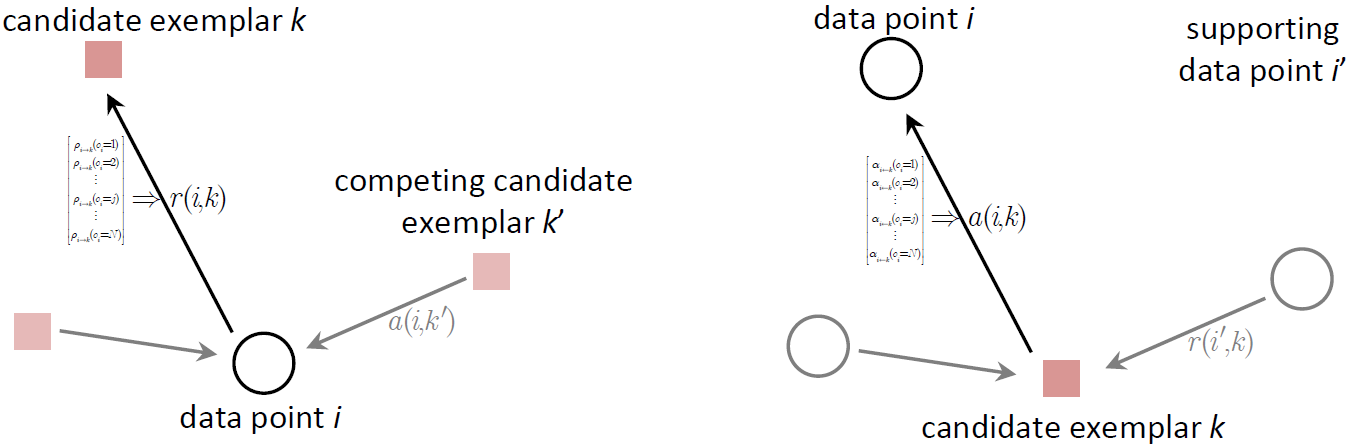
\includegraphics[width = 13 cm]{image/Chapters/Chapter2/APmessage.PNG}
    \caption{AP sends two types of message towards other data points: responsibility and availability \protect\cite{dueck2009affinity}. Responsibility $r(i,k)$, is the message from data $i$ to candidate exemplar $k$ and the respond back to figure out if point $k$ is well suited as an exemplar for point $i$.
    Availability $a(i,k)$, send a message from exemplar point $k$ to point $i$ to find how well it would be for point $i$ to choose point $k$ as an exemplar.}
    \label{abc}
    \end{figure}


  \item\textbf{Criterion matrix:} Lastly, in the criterion matrix, each cell is the sum of the availability matrix and responsibility matrix at that location. The highest criterion values of each row are designated as an exemplar.


\end{itemize}


The number of exemplar will end up with the number of clusters. Rows that have the same exemplar will be in the same cluster. The pseudo-code \ref{APo} shows the AP clustering algorithm.

\begin{algorithm}[]
    \SetKwInOut{Input}{Input}
    \textbf{Input:} Dataset $d=(d_{1}, d_{2},...,d_{n})$\\
    \textbf{Hyper-parameters:}
        {Preference, Damping, $conv_{it}, max_{iter}$}\\
\textbf{Output:} {Cluster centroids $C_1, ..., C_k$, branch points }\\
  	\SetKwFunction{FIROC}{AP}
    \SetKwProg{Fn}{Function}{:}{}
    \Fn{\FIROC{$d$}}{
        \textbf{Initialization:}\\
        {Similarity Matrix: S $\forall$ i, k:  s(i, k)} = 0\newline
        {Availability Matrix: A $\forall$ i, k:  a(i, k)} = 0\newline
        {Responsibility Matrix: R $\forall$ i, k:  r(i, k)} = 0\newline
        {Criterion Matrix: E $\forall$ i, k:  e(i, k)} = 0\newline
     \textbf{Compute S:}
        {$\forall i, k:  s(i, k) \leftarrow -\norm{V_i - V_k}^2 where V_i = (M_i, S_i) $}\newline
  	 \emph{
  	 \While{$r(i,k)$ $\&$ $a(i,k)$ \neq convergence}{
  	 \txt{Compute R:}\newline
  	       $r(i, k) \leftarrow s(i, k) - \max\limits_{k' s.t. k' \neq k}\{ a(i, k') + s(i, k')$ \}\newline
  	       \emph{Compute A:}\newline
  	       $a(i, k) \leftarrow \min\{0, r(k,k) + \sum\limits_{i' s.t. i' \notin \{i, k\}}{\max\{0, r(i',k) \}}$\newline
  	       no-diagonal A:\newline
  	       $a(i, k) \leftarrow \sum\limits_{i' \neq k}\max(0, r(i', k))$\\
  	       cluster assignment: $E = (E_1,..E_n)$ $E = argmax[a(i,k) + r(i,k)]$
  	       }  	    }
  	       
          	  }  \textbf{Results }C = $(C_1, ..., C_k)$
            
 \caption{Affinity Propagation Algorithm}
\label{APo}
\end{algorithm}





% The convergence of the algorithm is dependent on the damping parameter. Preference control the probability of finding exemplars. The probability increases with the increasing value of preference till a threshold is reached().

%The default values are listed below, which are used for our DSAP model during online and offline mode. These values work for our dataset and may vary based on the other data. Hyper-parameters are variables that control the performance and structure of any machine learning model. There are four main hyper-parameters that are used to control the performance of the proposed DSAP algorithm. Some of these parameters need to be defined at the start of the DSAP algorithm while a few are estimated based on the dataset under evaluation. These four hyper-parameters are:

Applying AP for any dataset requires to meet two condition: no missing or null data in the inputs and The data should be numeric, not categorical.
To improve the algorithm performance, hyper-parameters should be considered. These parameters are variables that control the performance and structure of any machine learning model and they are grouped in four, Preference, damping maximum iteration, and convergence iteration. These parameters are described below.
\begin{itemize}
    \item\textit{Preference parameter:}  Value determines how likely is a data point $i$ to be chosen as a centroid. This value is in the diagonal of similarity matrix. The number of identified clusters can be increased or decreased by changing this parameter correspondingly, and a good choice is to set the preference to be the median of all the similarities between data points \cite{li2012improved}.
    %This value for the e-counter dataset for the online phase is -4 and the value of the offline phase is -1. This number is a median value of the similarity matrix.
    \item\textit{Damping factor:}  is the extent to which the current data point is maintained relative to incoming data points. Damping should be between 0.5 to 1. 
    \item\textit{Maximum number of iteration:}  defines the maximum number of iterations. The default value for both online and offline phase is 100.
    \item\textit{Convergence iteration:}  is the number of iterations with no change in the number of estimated clusters that stop the convergence.
\end{itemize}
%elmi-In un-convergent cases, we have to increase lam manually and gradually and rerun AP until the algorithm converges. Another choice is to use a big damping factor close to 1 to eliminate oscillations, but AP will run very slow. Both choices may consume plenty of time, especially for a large data set
%    \item Number of initial data points: 500 items from the head of the stream
 %   \item Threshold($\epsilon$): This number is the average distance between data points and exemplars in the first phase. For e-counter dataset it is equal to 1.

%) preferences for each data point that is more likely to be chosen as an exemplar. 2) $convergence\_iter$ is the number of iterations with no change in the number of estimated clusters that stop the convergence. 3) damping factor (between 0.5 and 1) is the extent to which the current data point is maintained relative to incoming data points (weighted 1 = damping); and 4) $max\_iter$ defines the maximum number of iterations.







\subsection{K-means Clustering Algorithm} \label{kmeansalgo}
K-means Algorithm was first used by J.MacQueen in 1967 \cite{macqueen}, the process of partitioning population into $k$ orders and used the first k data as centroids to the closest centroid.
K-means is a partitioning and k centroids algorithm that aims to group $N$ observations into $k$ clusters in which each observation belongs to the cluster with the nearest center.

The K-means algorithm is formed of the following steps:
\begin{enumerate}
    \item Place k points in the space represented by the objects that are being clustered. These data points describe the initial set of centroids.
    \item Assign each data point to the group with the closest centroid.
    \item When all data points have been assigned to the closest group, the positions of the k centroids is being recalculated.
    \item Repeat Steps 2 and 3 until convergence (centroids no longer move).
\end{enumerate}




As can be seen from figure \ref{ite}, at first, cluster centers are initialized randomly or by applying heuristic techniques. Then, each data point is assigned to its closest centroid. 
In the next step,  the centroids are moved to the mean of each cluster's mapped points which ${\mu_k}$ is the mean of cluster $k$ :
\begin{equation}
    {\mu_k} = \frac{1}{{N_k}}\sum_{q=1}^{{N_k}} {x_q}
\end{equation}

%In this formula, $N_k$ is the number of instances belonging to cluster $k$
Finally, these process will be repeated until convergence. 

\begin{figure}
\centering
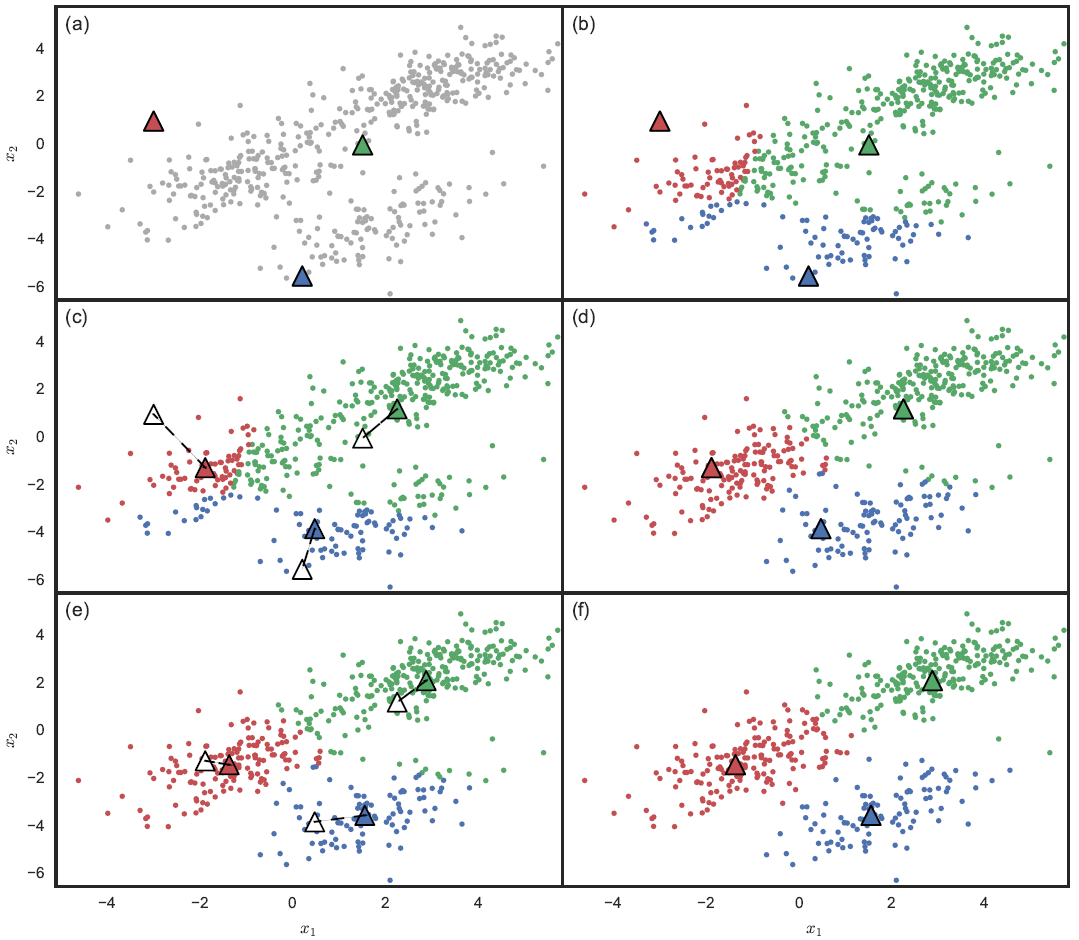
\includegraphics[width = 10 cm]{image/Chapters/Chapter2/kmeanshif.png}
\caption{K-means Algorithm: finding clusters in 2D space data during iterations \protect\cite{benavente2017automatic}. (a)cluster centroids initialization randomly, (b) data points map to the closest centroids, (c) centroids are moved to the mean of each cluster map points, (d,e,f) steps are repeated iteratively until convergence.}
\label{ite}
\end{figure}

The K-means algorithm starts with the K initial set of cluster-centers and iteratively updates it to decrease the error function. A proof of the finite convergence of the K-means type algorithms is given in \cite{selim1984k}. The complexity of n iterations of the K-means algorithm is O(n * K * m * N). Which n is a number of iterations, K set of macro clusters, m is the sample size with N attributes.  This linear complexity is one reason for the demand of the Kmeans algorithms. Even if the number of data points is considerably large, K-means is computationally efficient. 
Other reasons which make the algorithm so popular are a straightforward interpretation of clusters, simplicity of implementation, fast convergence, and adaptability to sparse data \cite{dhillon2001concept}.

 K-means is a partitioning algorithm that works well just on data with isotropic clusters and is not as versatile as single link algorithms.
Also, this algorithm is receptive to noisy data or outliers (one data point as an outlier can increase the squared error dramatically); it is suitable only when the mean is defined, and it needs the number of clusters prior, which is not easy when no prior information is available.
The  K-means algorithm is limited to numeric attributes. 
Figure \ref{kmAlgo} presents the pseudo-code of K-means algorithm.

\begin{figure}
\centering
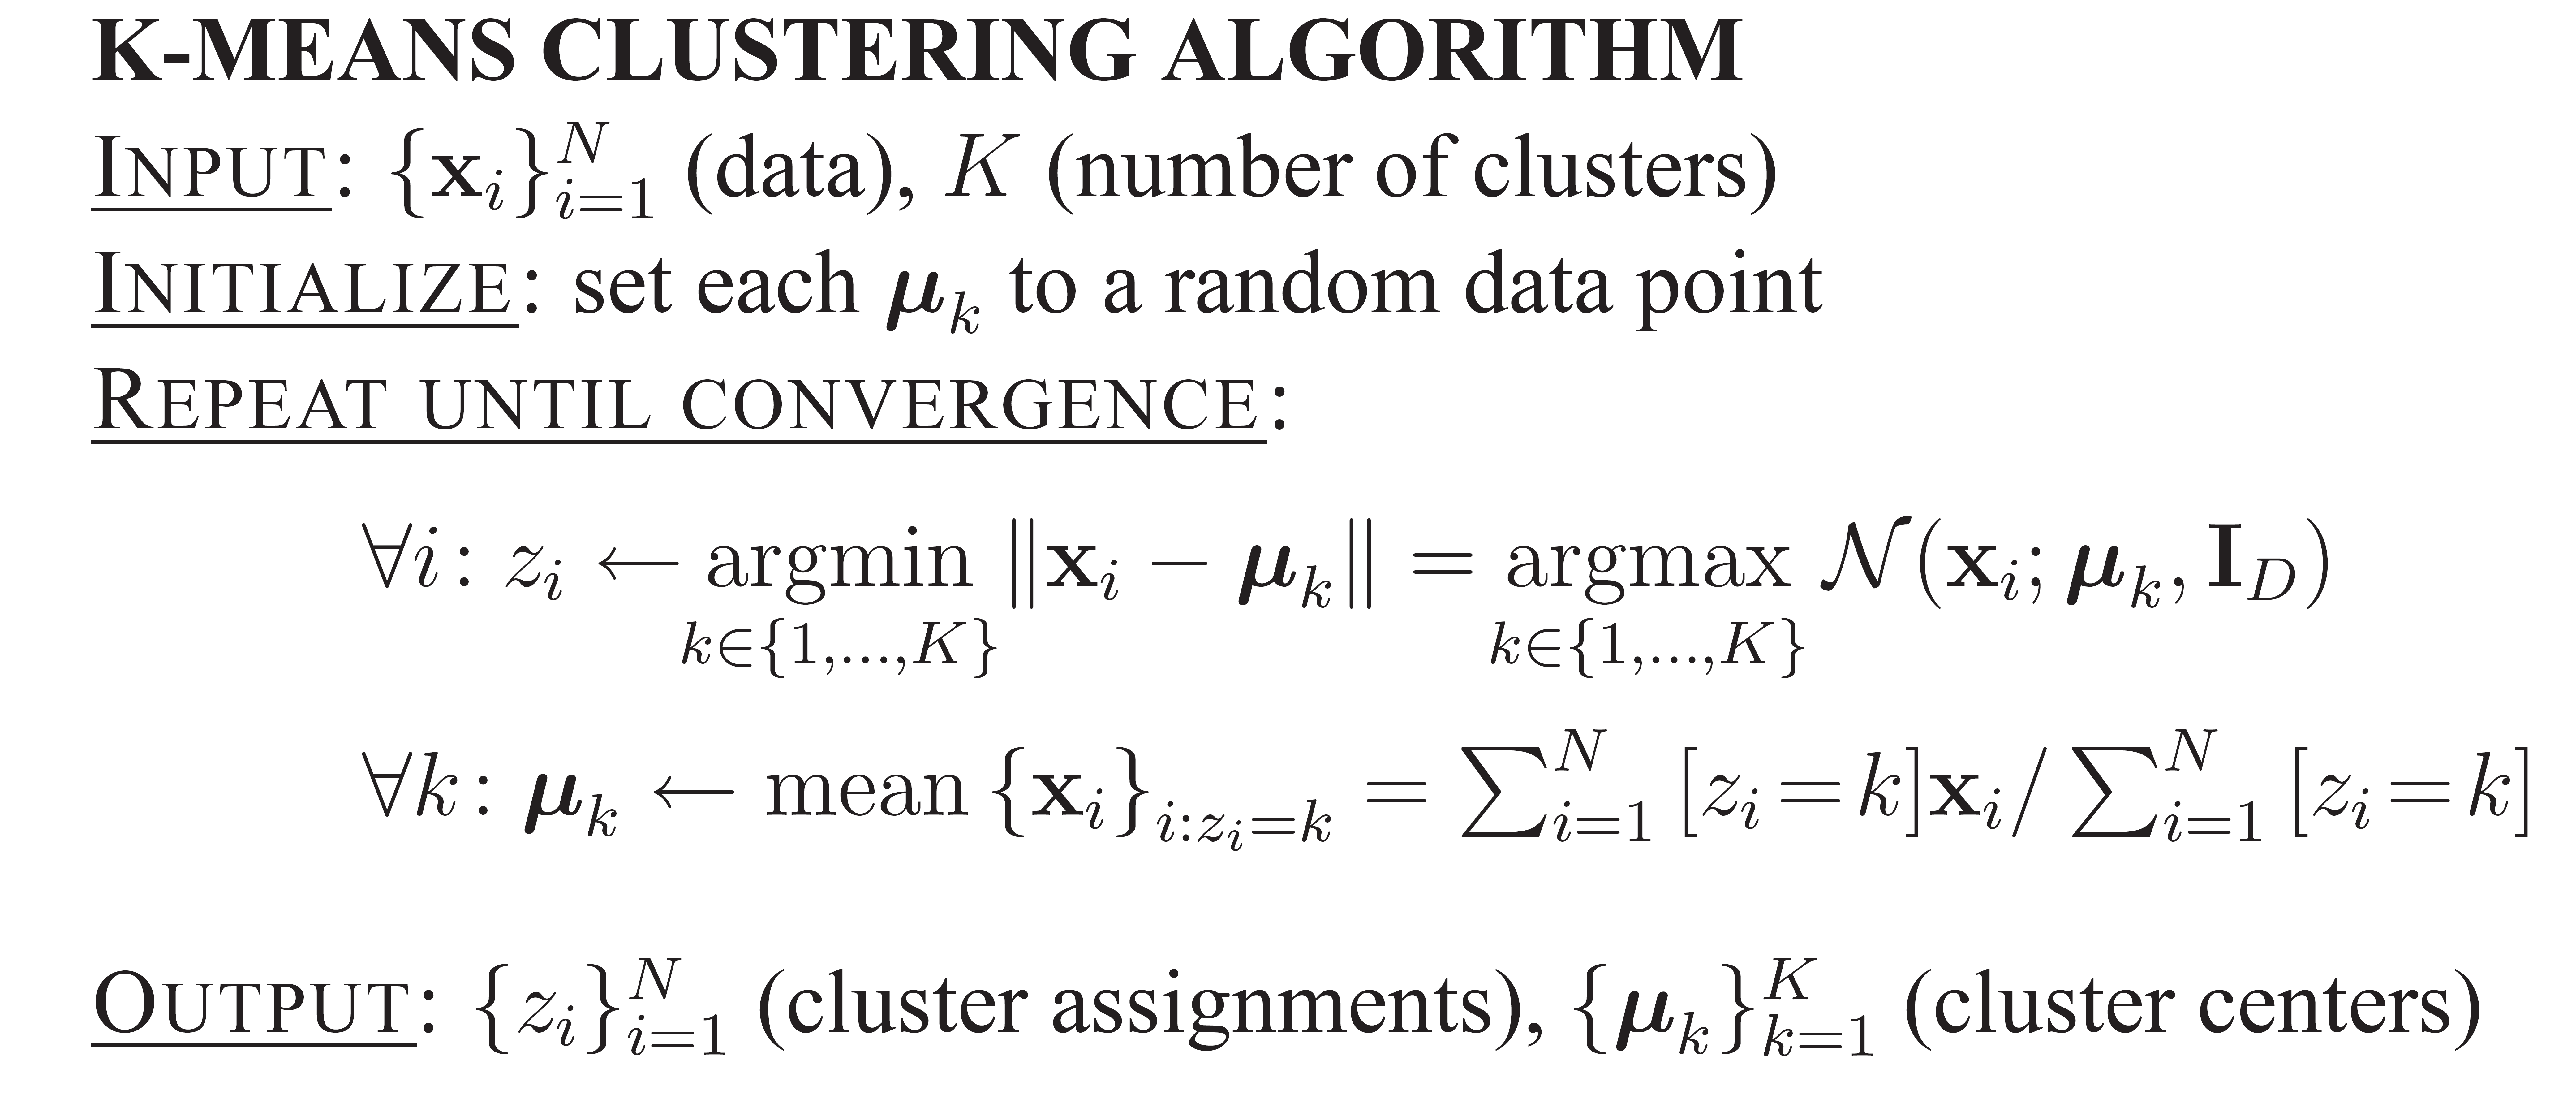
\includegraphics[width = 10cm,height = 4cm]{image/Chapters/Chapter2/6.png}
\caption{K-means pseudocode }
\label{kmAlgo}
\end{figure}


%%Elmi
% The similarity measure on numeric attributes is the square Euclidean distance; the similarity measure on the categorical attributes is the number of mismatches between objects and the cluster prototypes.

 %%%%%%%%%%%%%%%%%%%%%%%%%  ELMI

% A number of convergence conditions are possible. For example, the search
% may stop when the partitioning error is not reduced by the relocation of the centers.
% This indicates that the present partition is locally optimal. Other stopping
% criteria can be used also such as exceeding a pre-defined number of iterations.


% The Achilles heel of the K-means algorithm involves the selection of the initial partition. The algorithm is very sensitive to this selection, which may make the difference between global and local minimum.
% K-Means is one of the simplest unsupervised learning algorithms that solve the well known clustering problem. The procedure follows a simple and easy way to classify a given data set through a certain number of clusters (assume k clusters) fixed a priori.The main idea is to define k centroids, one for each cluster. These centroids should be placed in a cunning way because of different location causes different result. So, the better choice is to place them as much as possible far away from each other.The next step is to take each point belonging to a given data set and associate it to the nearest centroid. When no point is pending, the first step is completed and an early group is done. At this point, it is needed to re-calculate k new centroids as centers of the clusters resulting from the previous step. After these k new centroids, a new binding has to be done between the same data points and the nearest new centroid. A loop has been generated. As a result of this loop it may notice that the k centroids change their location step by step until no more changes are done. In other words centroids do not move any more.Finally, this algorithm aims at minimizing an objective function, in this case a squared error function. The objective function

% \begin{equation}
%     W(s,c) = \sum {k=1}^K\sum{iE S_k} \norm{y_i - c_k}^2
% \end{equation}
% Where S is a K-cluster partition of the entity set represented by vectors yi (iI) in the M-dimensional feature space,consisting of non-empty non-overlapping clusters Sk, each with a centroid ck (k=1,2,…K).
% ###############













%%%%%%%%%%%%%%%%%%%%%%%%%%%%%%%%%%%%%%%%%%%%%%%%%


There are several approaches to determine the number of clusters for K-means clustering algorithm such as elbow method, Silhouette score, information criterion approach or cross-validation \cite{kodinariya2013review}.



\noindent\textbf{Elbow Method:}

Elbow method is a technique for K-means algorithm to find the optimal number of clusters by fitting the model with the range of value for $k$. In this method assume the line chart is an arm, then the elbow or the point of inflection on the curve is the best fit for the model. The scoring parameter can be distortion, Silhouette, and Calinski or many other parameters. Distortion computes the average of squared distance from each point to its assign centroid. This distance is usually is a Euclidean distance. Silhouette calculates the mean of Silhouette coefficient of all data points. Calinski score computes the ratio of dispersion between and within clusters.



% \begin{figure}
% \centering
% 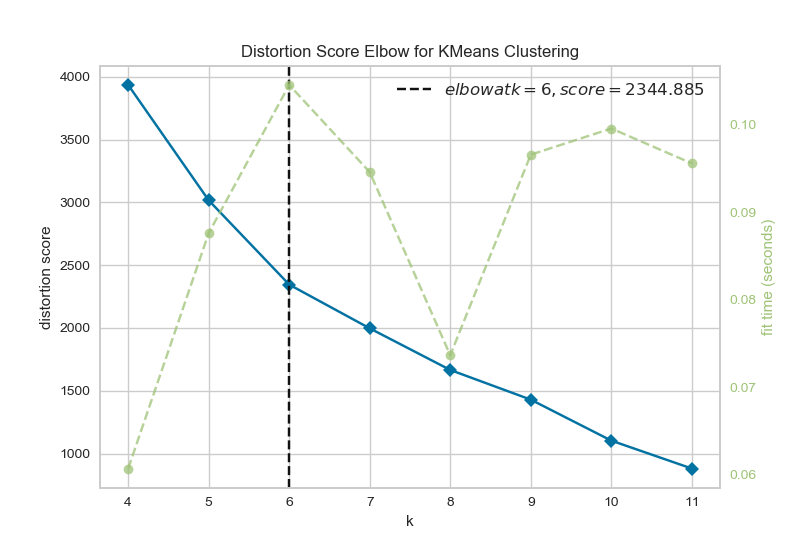
\includegraphics[width = 12cm,height = 8cm]{image/elbow.png}
% \caption{The elbow curve found for a $k$ range from 4 to 11 clusters. The black dotted line is the number of clusters determined by the elbow method}
% \label{elb}
% \end{figure}




\section{Data Stream Clustering }
\todo[inline]{SEQUENCE FOR THIS SECTION IS ONLINE/OFFLINE +  TIME WINDOWS +ALGORITHMS}

Data stream $S$ is sequence of real-time objects $d_1, d_2, ..., d_3 $ $\xrightarrow S = {d_i}$ which are infinitive,ordered, fast-changing at the rapid rates \cite{han2011data}.


In almost all clustering algorithms, the number of data points are fixed and evaluate each data point multiple times. However, many applications and systems generate observations continuously such as sensors, smart grids, network data, medical, finance and so on. In order to keep changes for new data points and the possible shift in cluster structures, classical clustering algorithms need to be run periodically. This method is computationally high and needs lot of data to be stored periodically. One major approach is to update existing clusters and merge new data points into the existing clusters by identifying emerging structures and removing outdated structures incrementally \cite{carnein2019optimizing}. This is the aim of data stream clustering algorithms which data points comes continuously in order and the stream is possibly unbounded.Finding the pattern without storing all the observations is a main task.
Data stream clustering finds clusters based on streaming and it is different from traditional clustering \cite{toshniwal2013clustering}:
\begin{itemize}
    \item Traditional clustering data are static, the data stream is dynamic.
    \item Traditional clustering datasets can be accumulated in memory but because of the enormous size of streaming data, it is not possible to store in memory.
    \item traditional clustering results are fixed but The data stream clustering results vary over time.
\end{itemize}


%The methods that discuss the problem of data stream clustering can be categorized into: (1) one-pass methods that assume a unique underlying model of streaming data and cannotmstudy the evolution of data distribution, (2) evolving clustering methods that take into account the behavior of data as it may evolve over time.

Many algorithms use similarity thresholds to decide whether an observation fits into an existing cluster or splitting the data space into a grid cells and store the location of dense or include fitting a model to represent the observed data. These categories and all related algorithms are shown in Figure \ref{method}, which divided in four main groups as follow \cite{zubaroglu2020data, ghesmoune2016state}. All these categories were reviewed in the cluster analysis section. 





\subsection{Two-phase Clustering Algorithms:}

All these approaches, capture the location of dense in the data space and considers as clusters. These clusters can be mergered when they become to similar over the time, however, it is not possible to split clusters again since the underlying data was discarded and only the centre of the dense region was remained \cite{aggarwal2007data}. To avoid this issue, many clustering algorithms models are divided in two parts: an online and an offline phases \cite{aggarwal2003framework}. Aggarwal introduced CluStream algorithm, combined online summarization at the first stage with the offline stage using k-means. The two-phase clustering methods are visualized in figure \ref{2phase} by the grid structure.

\begin{figure}
\centering
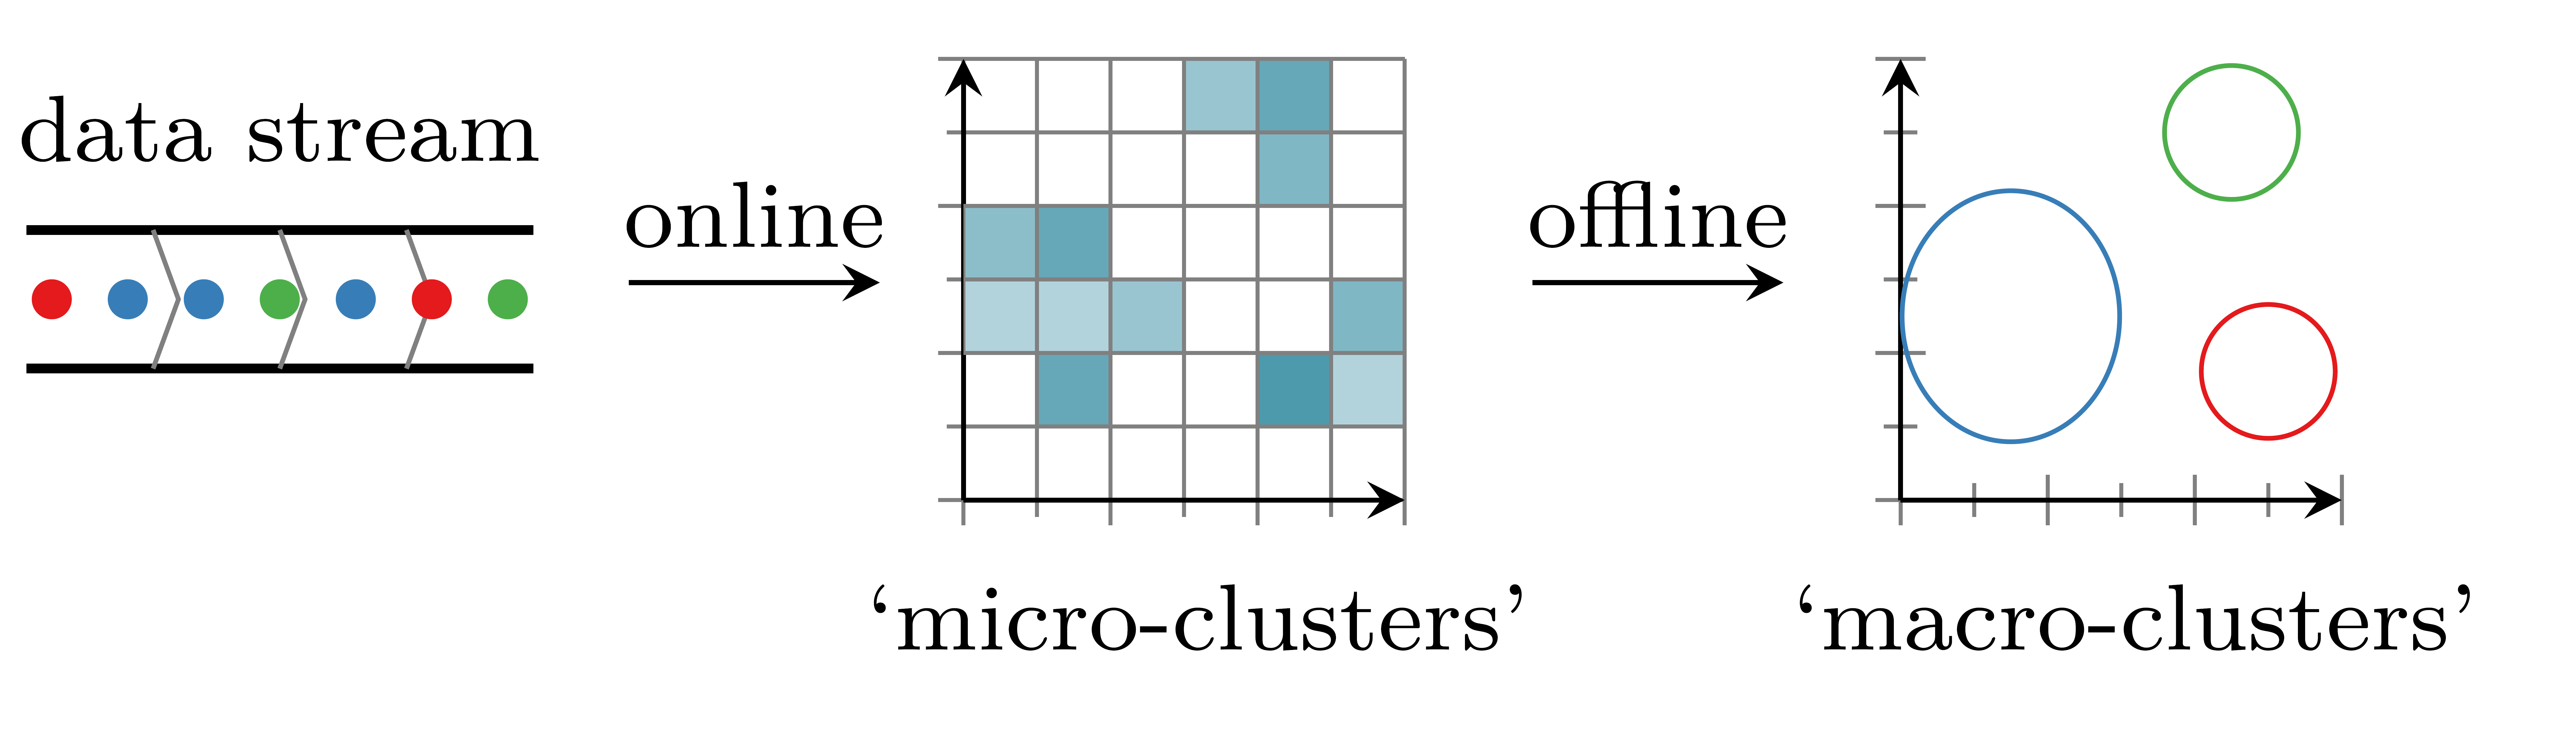
\includegraphics[width = 15cm,height = 4cm]{image/Chapters/Chapter2/2phase.png}
\caption{Simple overview of two-phase data stream clustering algorithms \protect\cite{carnein2019optimizing}.}
%\cite{carnein2017empirical} }
\label{2phase}
\end{figure}

The online requires a process for saving the summary statistics of a data stream in a fast manner. The offline phase uses the last stage summary statistics to provide the user with a fast understanding of the clusters whenever required. 

The offline component which can be based on the user request, it uses online micro clustering to find macro clusters by re-clustering the clusters obtained. this step is not time related and can be happen any time by the request. 


%The second phase is triggered at the end of a designated time interval. All the centroids of clusters which have been computed by using a sliding time window model, are re-clustered to create new macro clusters and centroids. The k-means algorithm is once again employed to compute the final $k_m$ macro clusters. The advantage of applying the macro-clustering is to gain further insight from the entirety of centroids after the designated streaming window. The optimal number of $k_m$ macro clusters can be calculated by using the same method as in micro cluster which is the elbow method. The elbow method calculation can be automated or estimated at the start of micro-clustering phase. This method works by applying the k-means algorithm on micro clusters computed for all sliding time windows. 


\subsection{Time Window Models:}
Due to data stream volume, it is impossible to store entire objects. To control which part of data is going to be processed, time window models have been proposed. The other reason to use time window model is to handle the concept-drift or data distribution over the time. It means This method aims to ignore outdated and historic data because they can change the trends or the data distribution.
Four main types of window models have been introduced. The most recommended models are damped window, landmark window, sliding window and tilted or pyramidal window model \cite{nguyen2015survey, mansalis2018evaluation}, which they are described in more detail below and illustrated in figure \ref{time1}:

\begin{figure}[!h]
\centering
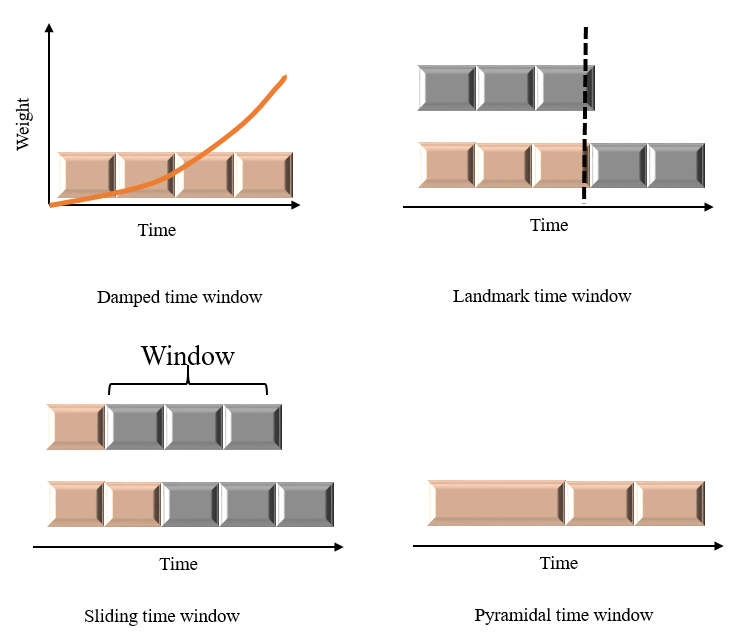
\includegraphics[width = 9cm,height = 7cm]{image/timeW.PNG}
\caption{Time Window Models.}
\label{time1}
\end{figure}



\begin{itemize}

    \item\textbf{Damped Time window:} It also referred as time-fading model, each data point has a different weight based on its arrival time so new data point has a higher weight than the old ones. This window model reduce the impact of old data. It is usually apply for density-based clustering algorithm. The Function: $f(\delta t)$ = $\mu_{\delta t}$ (0 < $\mu$ < 1) is usually used for this model where $\delta t$ is the age of data which is equal to time differentiation between current time and arrival time. A fading parameter $\mu$ is in the range between 0 to 1 \cite{nguyen2015survey}. 
    
    
    \item\textbf{Landmark Time Window:} Landmark time window or in-terms of implementation can be called as a hopping model, clustering starts from a starting point call landmark to the current time. When a new window comes, all data from the previous landmark are removed. In the landmark time window, each data point is equally important.


    
    \item\textbf{Sliding Time Window: } The most important data is the most recent ones and old data will be removed but the data in the current window are equally valuable. The data structure of sliding window is based on FIFO (First-In-First-Out) principle which data from current time until specific time in the past. The window has a size of $w$ in the current time $t$, will slide (s, sliding(w)) where s[t-w+1, t].
    The window size can be set based on resources and computational process \cite{silva2013data}.This model is efficient when most recent data is important \cite{mansalis2018evaluation}  
    
    \item\textbf{Pyramidal Time Window: } pyramidal or tilted time window focus on recent data without discarding old data. It applies various granularity levels based on the recency of data\cite{aggarwal2003framework, nguyen2015survey}. It stores almost all dataset and and prepare a balance between storage requirements and accuracy. This approach shows that current data are more accurate and should be fully modeled. The old data is aggregated and a generic representation is enough.
    
\end{itemize}    


\subsection{Data Stream Clustering Algorithm}
Data stream clustering algorithms are categorized in five main group as the traditional clustering algorithm mentioned before and illustrated in Figure \ref{method}. Some of these algorithms are described as follow.


\begin{figure}
    \centering
    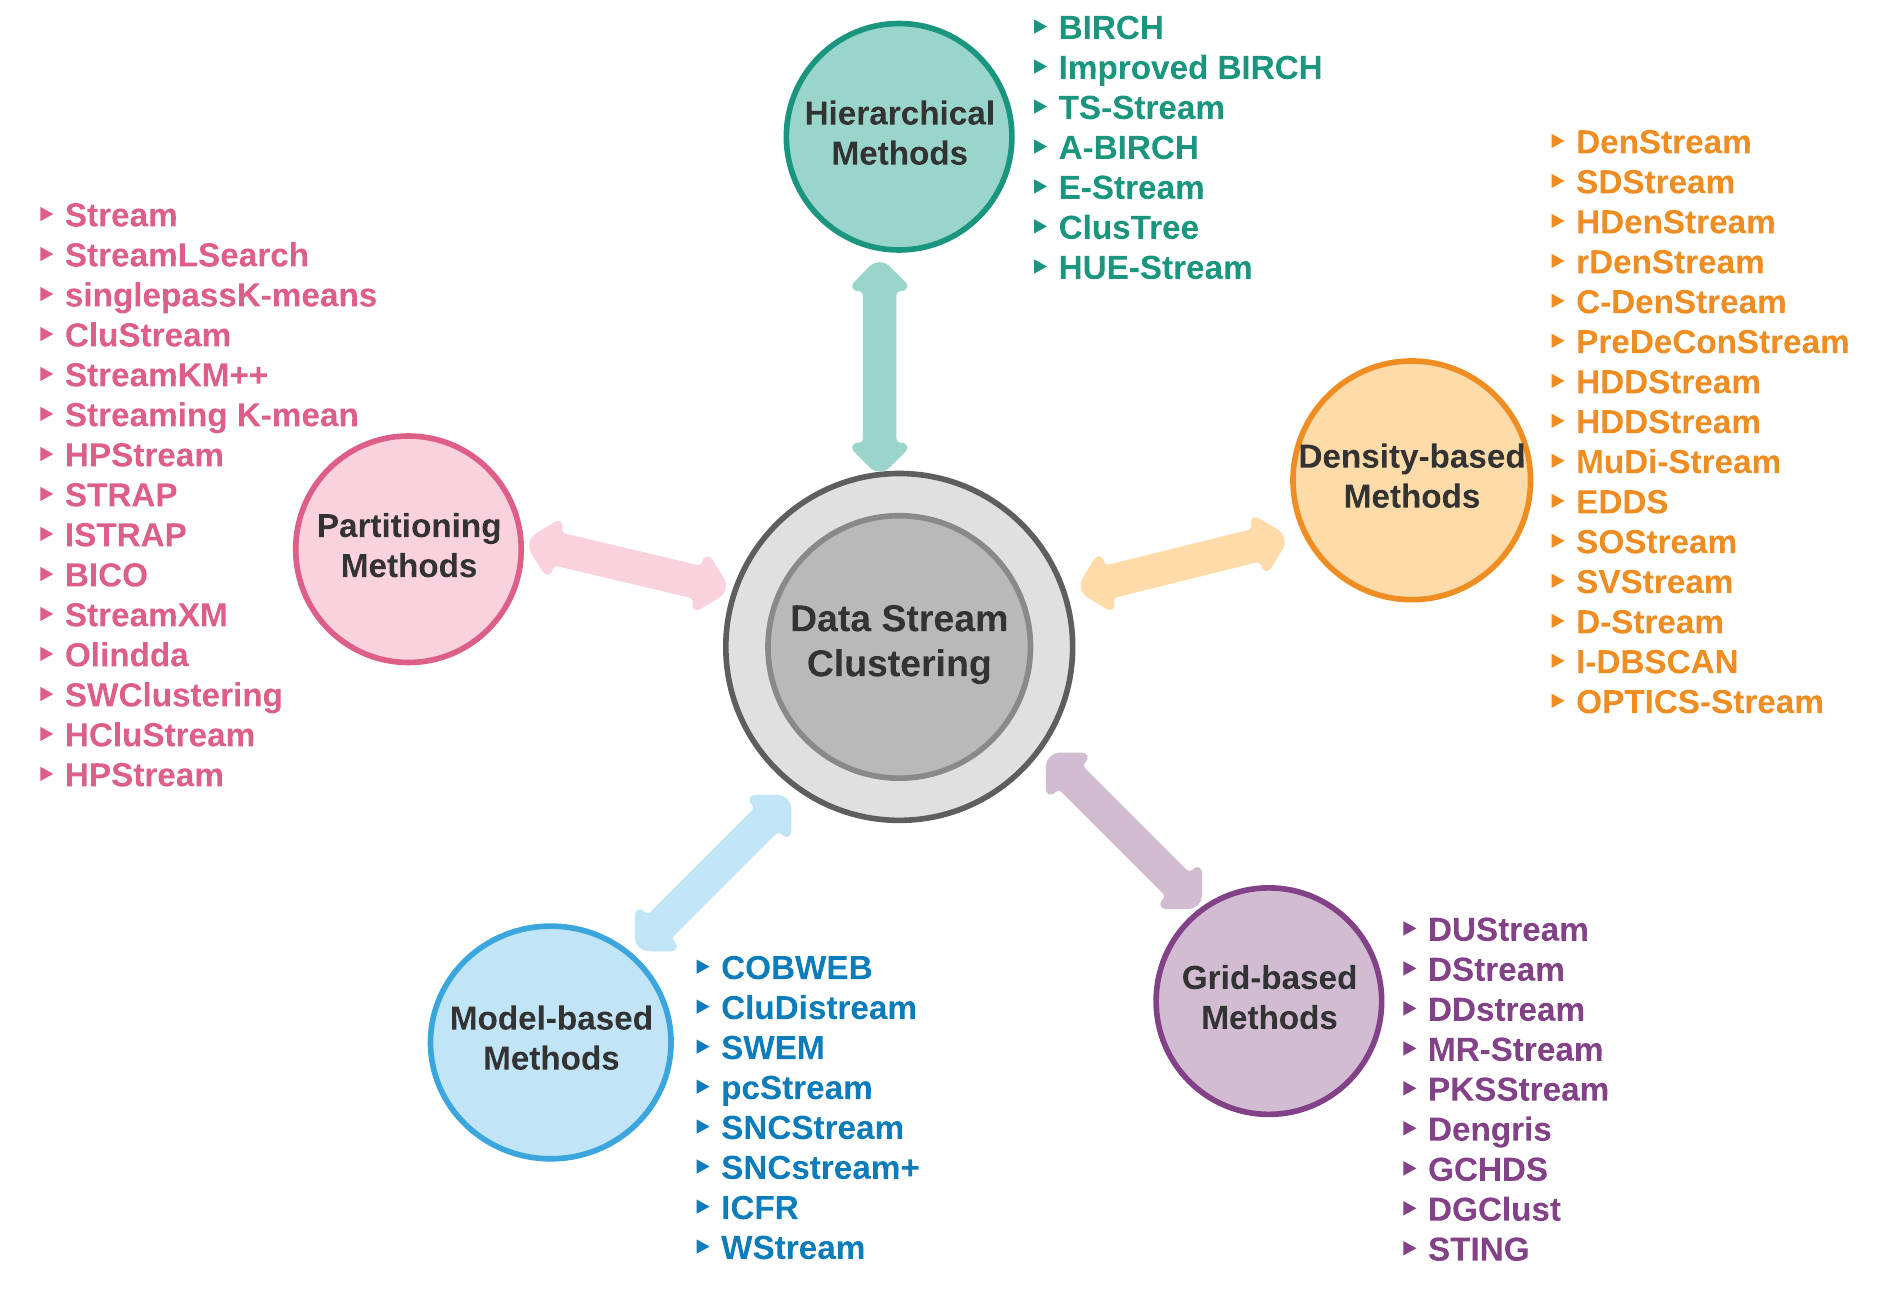
\includegraphics[width = 12 cm]{image/Chapters/Chapter2/streammethod.png}
    \caption{Data stream clustering algorithms categories}
    \label{method}
\end{figure}


\begin{itemize}
    \item\textbf{Partitioning algorithms:}


The First group is partitioning data stream clustering algorithm which they are listed in Table Table \ref{landmarkwin}. As far as we had research, there is not any research work present with affinity propagation used landmark time window model.


\begin{table}[h]
    \centering
    \caption{Overview of partitioning-based stream clustering algorithms implemented with the time window models \protect\cite{carnein2019optimizing, mansalis2018evaluation}. }
    \label{landmarkwin}
    \small
    \begin{tabular}{c c c c c}
    \hline
      \textbf{Algorithms} & \textbf{Year} & \textbf{ Method } & \textbf{Processing} & \textbf{ Time Window}  \\
     \hline \midrule

      Stream             &   2002        &   k-median        &  Single-pass      & Landmark \\
     \hline
     Olindda          &   2003        &   k-means         &   Single-pass     & Landmark \\
    \hline
     CluStream            &   2003        &  k-means       &  Online-Offline      & Pyramidal \\
    \hline   
     HCluStream           &    2006        &    k-means     &      & Pyramidal\\
    \hline    
     SWClustering       &    2008        &    k-means     &    Online-offline    & Sliding\\
       \hline
      StreamKM++       &    2012       &   k-means++ & Merge-reduce  & Landmark \\
    \hline 
      BICO               &    2013        &    k-means     &                     & Landmark\\
    \hline
     StreamXM            &   2015        &  x-means         &  merge-reduce      & Landmark \\
    \hline
    %  Stream K-means     &   2017        &  k-means         &  Online-offline      & Sliding/Damped \\
\bottomrule
    \end{tabular}
\end{table}



The Stream algorithm prposed by Guha et al. \cite{o2002streaming} is one of the earliest approach in this field. This method is k-median approach, and divides the stream into batches od data with the fix size. At each batch, k-median algorithm is applied. 


Olindda introduced by Spinosa \cite{spinosa2007olindda}, based on the K-means clustering algorithm is a online anomaly detection algorithm. Olindda continuously monitors and adapts to emerging data distributions. Unknown samples are kept in a memory queue, and are periodically clustered and then either merged with existing similar cluster or added as a novel cluster to the pool of clusters.
This model calculate the maximum distance between data points and centroids as a decision boundary (threshold) for each cluster. The union of the boundaries of all clusters is the global decision boundary which defines the model. A new unseen data point that falls inside this boundary is consistent with the model and therefore considered normal. Otherwise, This specific data point is labeled as an unknown and separated for further analysis.
%similar to my work
CluStream \cite{aggarwal2003framework} is inherited from BIRCH algorithm. The online phase is started by applying the k-means algorithm to create micro-clusters. When a new data point arrives, it is absorbed by its closest micro-cluster if it fit within an adaptive radius threshold. Otherwise, it creates a new cluster. To keep micro-clusters in some range, exppired clusters are removed based on a threshold on their average time stamp. If it cannot happen, the two closest micro-clusters will be merged.
To support different time-horizons, CluStream frequently collects snapshots of the current CFs by a pyramidal time frame. 

Another algorithm is HCluStream \cite{yang2006hclustream} is an extension of CluStream for categorical data by storing the frequency of attribute-levels for all categorical features. This algorithm creates a  categorical distance measure separately to combine with the traditional distance measure for continuous attributes.

SWClustering \cite{zhou2008tracking} introduced a new data structure for this algorithm called Exponential Histogram of Cluster Feature (EHCF) which can handle cluster evolution and represents the changes of the cluster distribution and capture it. In online phase, it captures objects as synopses in EHCF structure, and in offline phase, algorithm clusters these collections of synopses using a k-means algorithm.

Ackermann et al. \cite{ackermann2012streamk} develop a new coreset construction for the Euclidean k-means clustering problem and called it StreamKM++. A coreset is a small weighted point set that approximates the original input
point set with respect to a given optimization problem. This algorithm proposed a coreset construction for the Euclidean k-means clustering problem called coreset tree that is suitable for high dimensional data. Then, they used a standard streaming technique, called the merge-and-reduce technique to maintain observation in data streams. After processing the whole input stream, the k-MEANS++ algorithm applies to obtain a k-means clustering and celled it StreamKM++ algorithm.

BICO \cite{fichtenberger2013bico} is another algorithm in this group which combines the BIRCH data structure with StreamKM++. 






\item\textbf{Hierarchical-based algorithms:}

\begin{table}[h]
    \centering
    \caption{Overview of Hierarchical-based stream clustering algorithms. }
    \label{hirarcha}
    \small
    \begin{tabular}{c c c c c}
    \hline
      \textbf{Algorithms} & \textbf{Year} & \textbf{ Method } & \textbf{Processing} & \textbf{ Time Window}  \\
     \hline \midrule

      BIRCH             &    1996        &     CF-tree  &  Single-pass       & Landmark \\
     \hline
     Improved BIRCH     &    2014        &    CF-tree   &    Single-pass     & Landmark \\
      \hline
      TS-Stream         &     2015       &    -      &     Decision tree  & Sliding  \\
    \hline 
      A-BIRCH           &    2017        &   CF-tree    &   Single-pass      & Landmark\\
\bottomrule
    \end{tabular}
\end{table}

BIRCH \cite{zhang1996birch} is one of the earliest stream clustering algorithm. This algorithm minimizes large datasets' memory requirements by summarizing the information contained in dense regions as Clustering Feature (CF) entries. CF has three components: number of data points, the d-dimensional vector with the linear sum of all data points, and sum of squares for all data points across dimensions. BIRCH incrementally builds a balanced-tree to maintain CFs, where each node can contain a fixed number of CFs. 
For every new data point that comes into the model, the tree descends by following the child to its closest CF until a leaf node is reached. The new data point can either merged to its closest leaf-CF or creates a new leaf-CF. This method has a significant drawback which is the limited capacity of its leaves.

Improved BIRCH \cite{ismael2014improved} is an extension of the BIRCH algorithm, which employs various distance thresholds per CF.

TS-Stream \cite{pereira2014ts} is a time-series data stream clustering with the time frame. 

A-BIRCH \cite{lorbeer2016birch} is similar to Improved BIRCH, determines the threshold parameters by using the Gap Statistics on a representation of the stream.



\item\textbf{Density-based algorithms:}

\begin{table}[h]
    \centering
    \caption{Overview of Density-based stream clustering algorithms. }
    \label{densalgo}
    \small
    \begin{tabular}{c c c c c}
    \hline
      \textbf{Algorithms} & \textbf{Year} & \textbf{ Time window } & \textbf{Method} & \textbf{ Processing}  \\
     \hline \midrule

      DenStream          &    2006        &    Damped          &    DBSCAN      & Online-offline \\
     \hline
     SDStream            &    2009        &    Sliding         &    DBSCAN      & Online-offline \\
      \hline
      HDenStream         &     2009       &     Damped         &    DBSCAN      &  Online-offline \\
    \hline 
      FlockStream        &    2009        &     Damped        &     Swarms      & Single-pass\\
    \hline 
      rDenStream         &    2009        &    Damped         &     DBSCAN      & Online-offline \\
          \hline 
      C-DenStream        &    2009        &    Damped         &     C-DBSCAN    &Online-offline \\
          \hline 
      PreDeConStream     &    2012        &   Damped          &     DBSCAN      & Online-offline\\
          \hline 
      HDDStream          &    2012        &   Damped          &     DBSCAN      & Online-offline\\
          \hline 
      EDDS               &    2017        &   Damped          &     DBSCAN      & Online-offline\\
\bottomrule
    \end{tabular}
\end{table}

DenStream \cite{cao2006density} is the temporal extension of the CFs from BIRCH algorithm with having core micro cluster using time-faded CF. This algorithm was implemented with arbitrary shape data.

SDStream \cite{ren2009density} is a variant of DenStream algorithm for sliding time window model. This algorithm keeps CMCs in the form of Exponential Histogram.
 
HDenStream \cite{lin2009density} is a combination of DStream (with the categorical distance measure ) and HCluStream for categorical datasets. 

FlockStream \cite{forestiero2013single} applies a flocking behavior to identify emerging flocks and swarms of objects. Like the DenStream algorithm, FlockStream differentiates between potential core and outlier micro-clusters and uses a time-faded CF. 

rDenStream \cite{liu2009rdenstream} to detects outliers,  this algorithm temporarily stores them away in an outlier buffer.  After the offline phase, the algorithm tries to re-cluster the data points cached in the buffer to improve the clustering.

C-DenStream \cite{ruiz2009c} is another type of  DenStream that allows domain knowledge in instance-level constraints into the clustering method. Instance-level constraints mean data points that can or cannot belong to the same cluster.

PreDeConStream \cite{hassani2012density} was implemented simultaneously to HDDStream. The algorithm changes in regular intervals by applying a modified PreDeCon algorithm on the micro-clusters generated during the online phase.

% HDDStream \cite{ntoutsi2012density}

\item\textbf{Grid-based algorithms:}
Grid-based algorithms are capture the density in the grid. Macro-clusters are usually obtained by grouping adjacent dense cells. How to make a grid cell is very challenging. Table \ref{gridd} shows the overview of some main algorithms in this group. The most popular grid-based algorithm is DStream \cite{chen2007density}.


\begin{table}[h]
    \centering
    \caption{Overview of grid-based stream clustering algorithms. }
    \label{gridd}
    \small
    \begin{tabular}{c c c c c}
    \hline
      \textbf{Algorithms} & \textbf{Year} & \textbf{ Method } & \textbf{Processing} & \textbf{ Time Window}  \\
     \hline \midrule

      Fractal Clustering &    2000        &           &  Single-pass        & Landmark\\
          \hline 
     DUstream            &    2005        &      Dense-unit       &     Single-pass     &  Landmark\\
      \hline
      Dstream            &     2007       &    Dense-region       &  Online-offline     &   Damped\\
    \hline 
      DDStream           &    2008        &    DCQ-means          &     Online-offline  & Damped \\
    \hline 
      MR-Stream          &    2009        &     Dense-region      &  Online-offline     & Damped\\
    \hline 
      PKS-Stream         &    2011        &    Dense-region       &  Online-offline     & Damped\\
          \hline 
      DENGRIS            &    2012        &   Dense-region        &  Single-pass        & Sliding\\
          \hline 
      HDCStream            &    2014        &           &    Single-pass      & Damped\\
          \hline 
      MuDi-Stream        &    2016        &       DBSCAN          & Online-offline      & Damped\\
\bottomrule
    \end{tabular}
\end{table}

Dstream has a fix grid size, with three different types of cells: dense cells, sparse cells, and transitional cells, which it is categorized between the other two types. The algorithm outlines new data points to its corresponding cell and is initialized by assigning all dense cells to individual clusters. These clusters are extended with all neighboring transitional grids or merged with neighboring dense cell clusters. In any intervals, the clustering assesses the weight of individual cell and includes the
changes in cell types into the clustering.


DUstream \cite{gao2005incremental} devides the data space once into fixed grid-cells.
The algorithm processes the first part of data to start the clustering and maintains all cells with sufficient density. The density of cells is determined, corresponding to the total number of observations. 

DDstream \cite{jia2008grid} is an extension on points that lie precisely on the grid boundaries. For these points, the distance to adjacent cell centers is calculated, and those points are assigned to their closest cell. 





\item\textbf{Model-based algorithms:}
This group of algorithms summarize the data stream as a statistical model, usually based on Expectation Maximization (EM) algorithm. 

\begin{table}[h]
    \centering
    \caption{Overview of model-based stream clustering algorithms. }
    \label{modealgo}
    \small
    \begin{tabular}{c c c c c}
    \hline
      \textbf{Algorithms} & \textbf{Year} & \textbf{ Method } & \textbf{Processing} & \textbf{ Time Window}  \\
     \hline \midrule

      COBWEB             &    1987        &   tree-based          &          & Landmark \\
     \hline
     WStream             &    2004        &   Kernel-density          &                     & Damped \\
      \hline
      CluDistream        &     2007       &   EM      &        &  Landmark \\
    \hline 
      SWEM               &    2009        &  EM         &  Online-offline      & Sliding\\
    \hline 
      SVStream          &    2013        &    SVC       &                     & Damped  \\
    \hline 
      pcStream          &    2015        &       SIMCA      &          Single-pass           & Damped  \\
\bottomrule
    \end{tabular}
\end{table}


COBWEB \cite{fisher1987knowledge} is a tree-based algorithm and each node describe a cluster. Tree incrementally builds by descending a new entry from the root to a leaf. 

WStream \cite{tasoulis2006unsupervised} uses kernel density to keeps a number of windows in the data space. It means to use local maxima of a density estimate as cluster centers and the local minima as cluster boundaries. New data points can add to an existing window or it is used to initialize a new window with the default size. 

CluDiStream \cite{zhou2007distributed} applies EM algorithm for data stream clustering. This algorithm learns the distribution of underlying data streams by maximizing the likelihood of the data clusters. It keeps distribution of Gaussian mixture and a coordinator node in each location to combine the distributions.

SWEM \cite{dang2009based} uses EM to chunks of data with random initial parameters. Distributions for the first chunk of data calculates. Each cluster is then summarized using a CF and macro-clusters by applying EM again.

SVStream \cite{wang2011svstream} is based on support vector clustering (SVC) which transform the data into the higher dimensional space. The model is run on chunks, and the first one runs SVC. For other chunks it checks if it is in the radius of spheres or not. If yes, a new sphere is initialize. 






\end{itemize}





   	    
%%%%%%%%%%%%%%%%%%%%%%%%%%%%%%%%%%%%%%%%%%%%%%%%%%%%%%%%%%%%%%%%%%%%%%%%%%%%%%%%%%%%%%%%%%%%%%%%%%%%% 

% \begin{algorithm}[H]
% \SetAlgoLined
% \textbf{Input:} Data stream $S=(s_{1}, s_{2},...,s_{n})$, number of micro clusters $k$, number of macro cluster $k_m$, sliding time window $W$ with the size $z$;\\
% \textbf{Output:} {Set of micro clusters $C_m= (C_{m_1}, C_{m_2}, ..., C_{m_k})$, and set of macro clusters $C_M= (C_{M_1}, C_{M_2}, ..., C_{M_{k_m}})$ }\\
% \SetKwFunction{FIROC}{Streaming K-means}
% \SetKwProg{Fn}{Function}{:}{}
% \Fn{\FIROC{S, W}}{
         
% \textbf{Initialization:}
% \begin{itemize}
%     \item Partition S with $W$ into k subsets $S_1$, . . . , $S_k$, such that $S_i$, 1 $\leq$ i $\leq$ k,
%     \item Extract $W_1$ = $(s_1...s_z)$ data points from $S$
%     % \item partition S with $W$ into k subsets $S_1$, . . . , $S_k$
%     \item Estimate $k$ initial centroids $c_1, . . . , c_k$ from $W_1$ using K-means
% \end{itemize}

% \Repeat{Centroid convergence is achieved}{          
%  \SetKwFunction{FIROC}{K-means}         \hfill \Comment{Online Phase}\\
% \SetKwProg{Fn}{Function}{:}{}
% \Fn{\FIROC{Wi,k}}{
%  Assign data points $s_i$ to the closest centroid\\
%  Replace the current centroids by new centroids $c_1, ..., c_i$\\}
% \textbf{return}{ $(C_{m_1}, C_{m_2}, ..., C_{m_k})$ }\\
% }

% \Repeat{Centroids convergence happens}{
%   \SetKwFunction{FIROC}{K-means}         \hfill \Comment{Offline Phase}\\
% \SetKwProg{Fn}{Function}{:}{}
% \Fn{\FIROC{C_m,k_m}}{                                     
%   Find $k_m$ macro clusters from $C_m$ centroids\\
%   }
% }

% \textbf{return} {macro clusters: $C_{M_1}, C_{M_2}, ..., C_{M_{k_m}}$\\ }
% }
%  \caption{Streaming K-means Online Micro and Offline Macro Clustering Algorithm}
% \end{algorithm}


%New ideas continue evolving in data streams over time. Evolving needs updating data stream algorithms to adjust to the changes such as handle well rapid cluster evolution patterns.







%%%%%%%%%%%%%%%%%%%%%%%%%%%%%%%%%%%%%%%%%%%%%%%%%%%%%%chapter 4
% \section{online- offline clustering}
% This section introduced a three phase, online micro, offline macro, and evaluation streaming K-means algorithm for comparison with the proposed DSAP algorithm. The streaming K-means algorithms are  widely used to analyze streaming data. In this section, the framework of streaming K-means algorithm is discussed. As shown earlier in Figure \ref{wrk1} the DSAP and streaming K-means algorithms have analogous phases with the major differences in the clustering algorithm.
% \subsection{Online Micro-Clustering Phase}
% In this phase, the data stream arrives are accumulated using the sliding time window model. The streaming K-means model incrementally updates when a new data window comes into the model to generate the micro clusters. These points can also be clustered using K-means with preferred $k$ cluster centroids. The approach used for selecting the $k$ number of micro clusters is the elbow method described previously in section \ref{elbowmethod}. The algorithm randomly chooses $n$ data points in each time frame until convergence happens. It computes the sum of the squared distances from each data point to its assigned centroid.

% \begin{figure}
% \centering
% 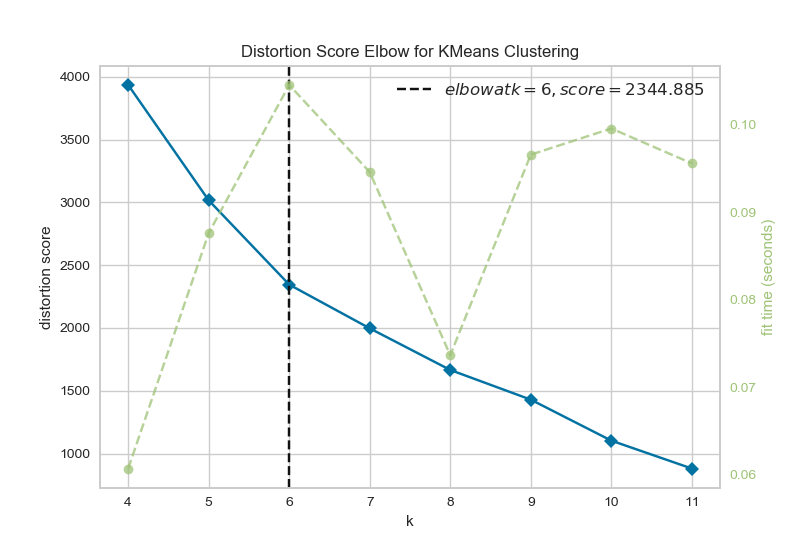
\includegraphics[width = 12cm,height = 8cm]{image/elbow.png}
% \caption{The elbow curve found for a $k$ range from 4 to 11 clusters. The black dotted line is the number of clusters determined by the elbow method}
% \label{elb}
% \end{figure}




%\subsection{Streaming K-means Clustering Performance Evaluation}
%The quality and efficiency of the streaming K-means clustering algorithm need to be evaluated as well as the DSAP algorithm. The quality of clusters found by each algorithm are assessed by these four criteria: Silhouette Coefficient, Calinski-Harabasz Index, Davies-Bouldin Index and outlier detection.
%The efficiency is compared using three metrics: computational time efficiency, frequency of the outliers and the memory consumed to run the program.



%\subsubsection{Evaluation of Data Stream Clustering}

%In data stream clustering (DSC) phase, stream currently provides moving windows and sampling from a stream as data stream operators.DSC\_Window provides a clustering interface to the data stream. It implements the sliding window and the dampened window models which keep a user-specified number (window length) of the most recent data points of the stream. For the dampened window model, data points in the window have a weight that deceases exponentially with age.
%%%elmi
%Evaluating the performance of a clustering algorithm is not counting the number of errors or accuracy. In particular, any evaluation metric if this clustering defines separations of the data similar to some ground truth set of classes or satisfying some assumption such that members belong to the same class are more similar than members of different classes according to some similarity metric.The main purpose of clustering methods is to find high intra-cluster similarity and low inter-cluster similarity. In a simple term, objects in the same cluster are more similar than the objects in different clusters.
%%




%%%%%%%%%%%%%%%%%%%%%%%%%%%%%%%%%%%%%%%%%%%%%%%%%%%%%%%%%%%%%%%%%%%%%%%%%%%%%%% KEEP
% \section{Sliding Time Window Model}
% The sliding time window model limits the scope of data to a sequence of the most recent data points in the data stream to compute the micro clusters, since the new data point is available, the old one is removed.
% The first window is started with a pre-defined time frame based on the data, and this window containing the accumulated data points from where the stream started. After a new data point arrives, the algorithm updates the micro clusters incrementally each time. Next, the new time window employs all the new data points and clusters as the data points, saving the new micro clusters and the selected centroids. 

% By applying a sliding time window model, the sum of square distances will often eliminate at a local optimum. Accordingly, it leads to the micro-clustering evolution results. The main focus is finding micro clusters evolution to identify new clusters from outliers. There are two types of sliding windows, time-based and count-based sliding windows \cite{li2014parallel}. In time-based sliding windows, time intervals are applied(e.g., every 10 minutes), while in count-based sliding windows, they are defined in terms of the number of data points. Figure \ref{stw} shows sliding time window model with the data points included in a window.  Equation \ref{eq11} shows the calculation of time window:
% \begin{equation}
%     W_i = [m_i, ..., m_{(i+w-1)}]\label{eq11}
% \end{equation}

% Where $w$ is a window length, $m_i$ is the $i^{th}$ data point and $W_i$ is the $i^{th}$ window. 
% \begin{figure}
% \centering
% %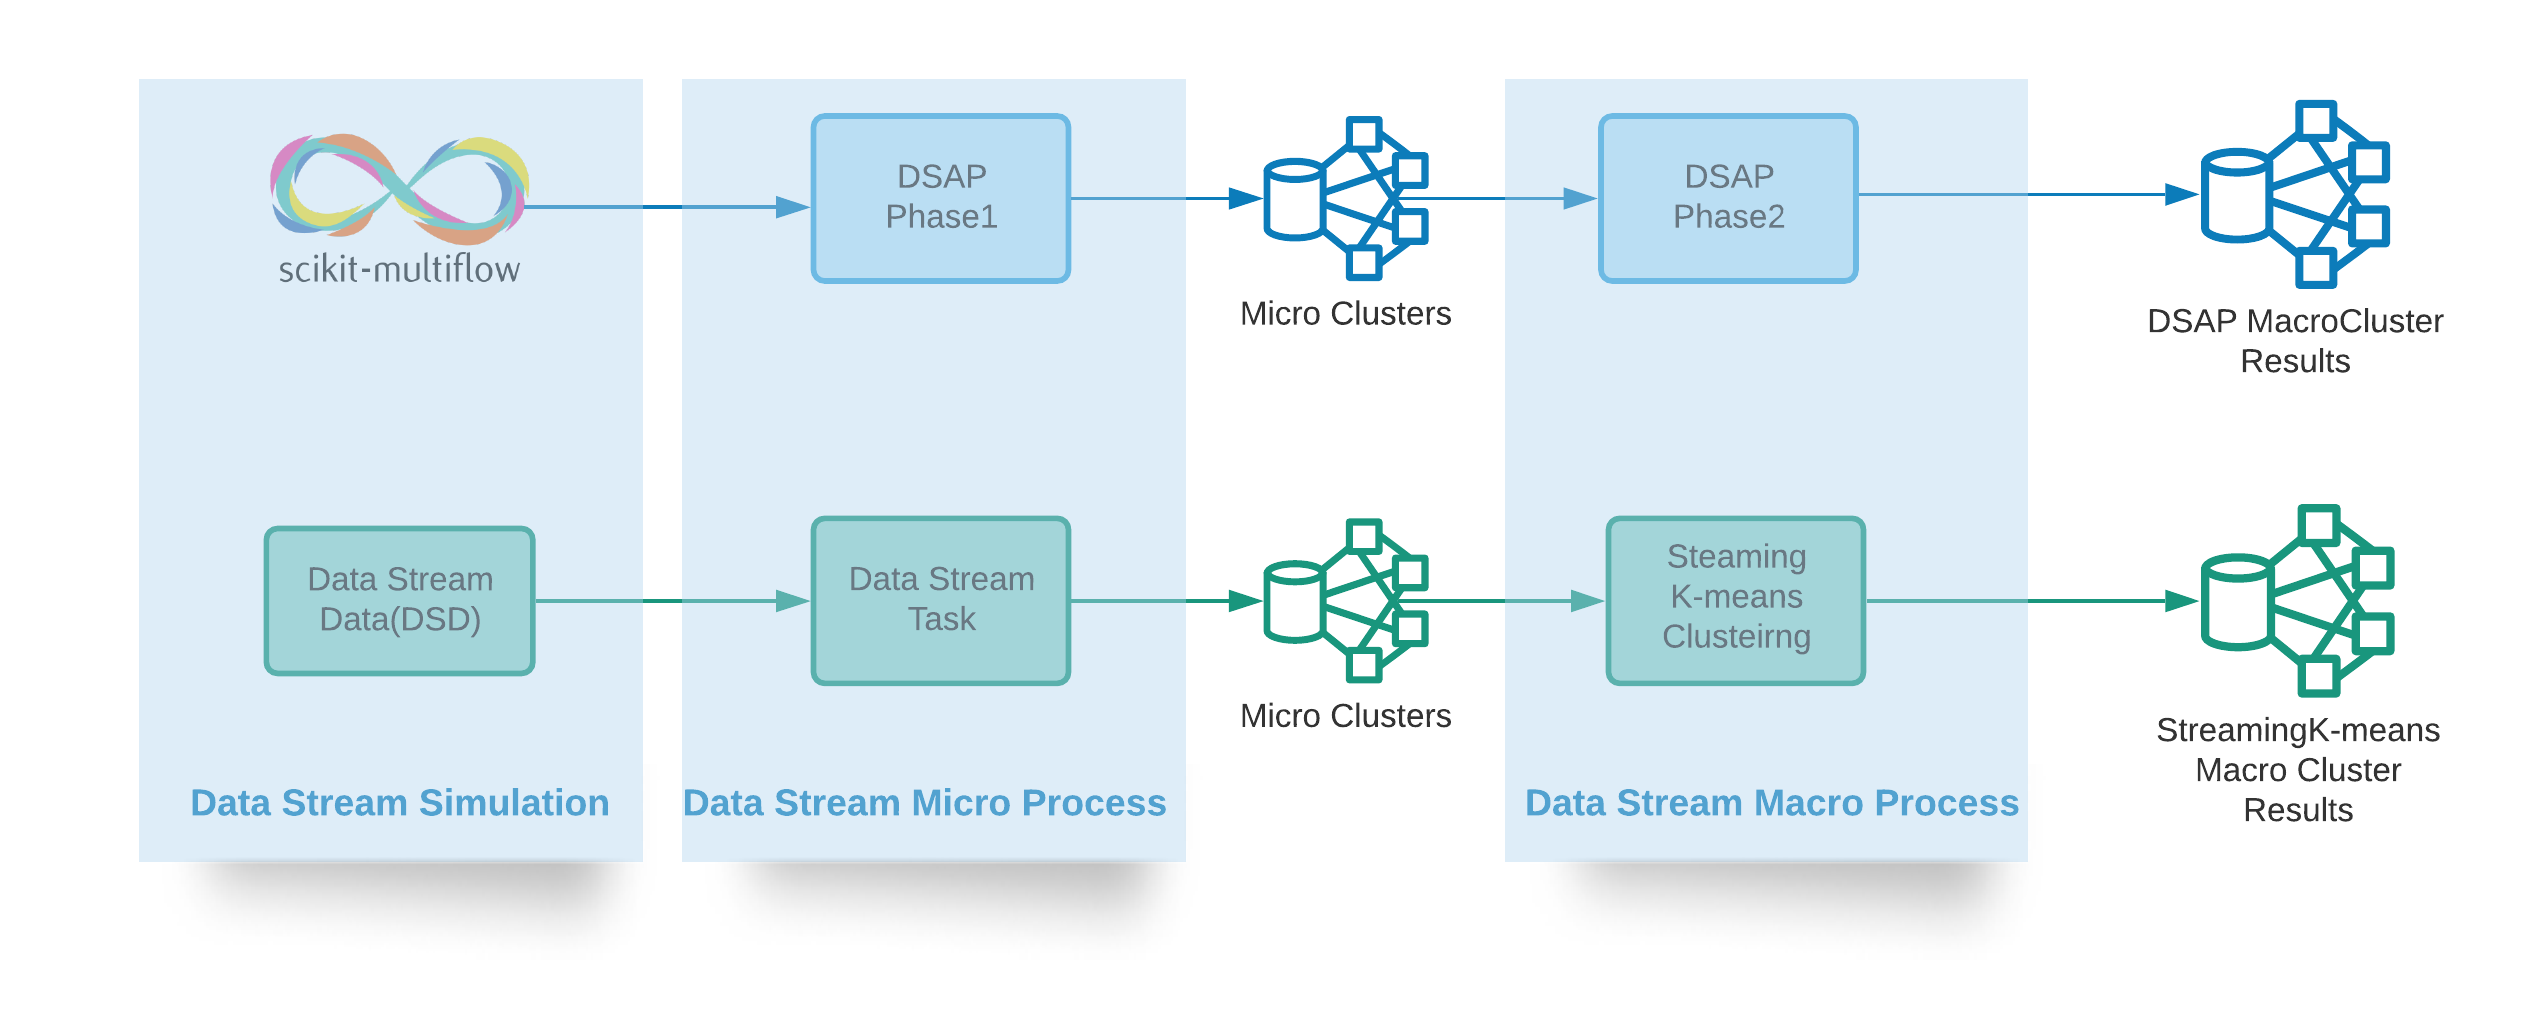
\includegraphics[width = 15cm,height = 7cm]{image/2-2workflow.png}
% 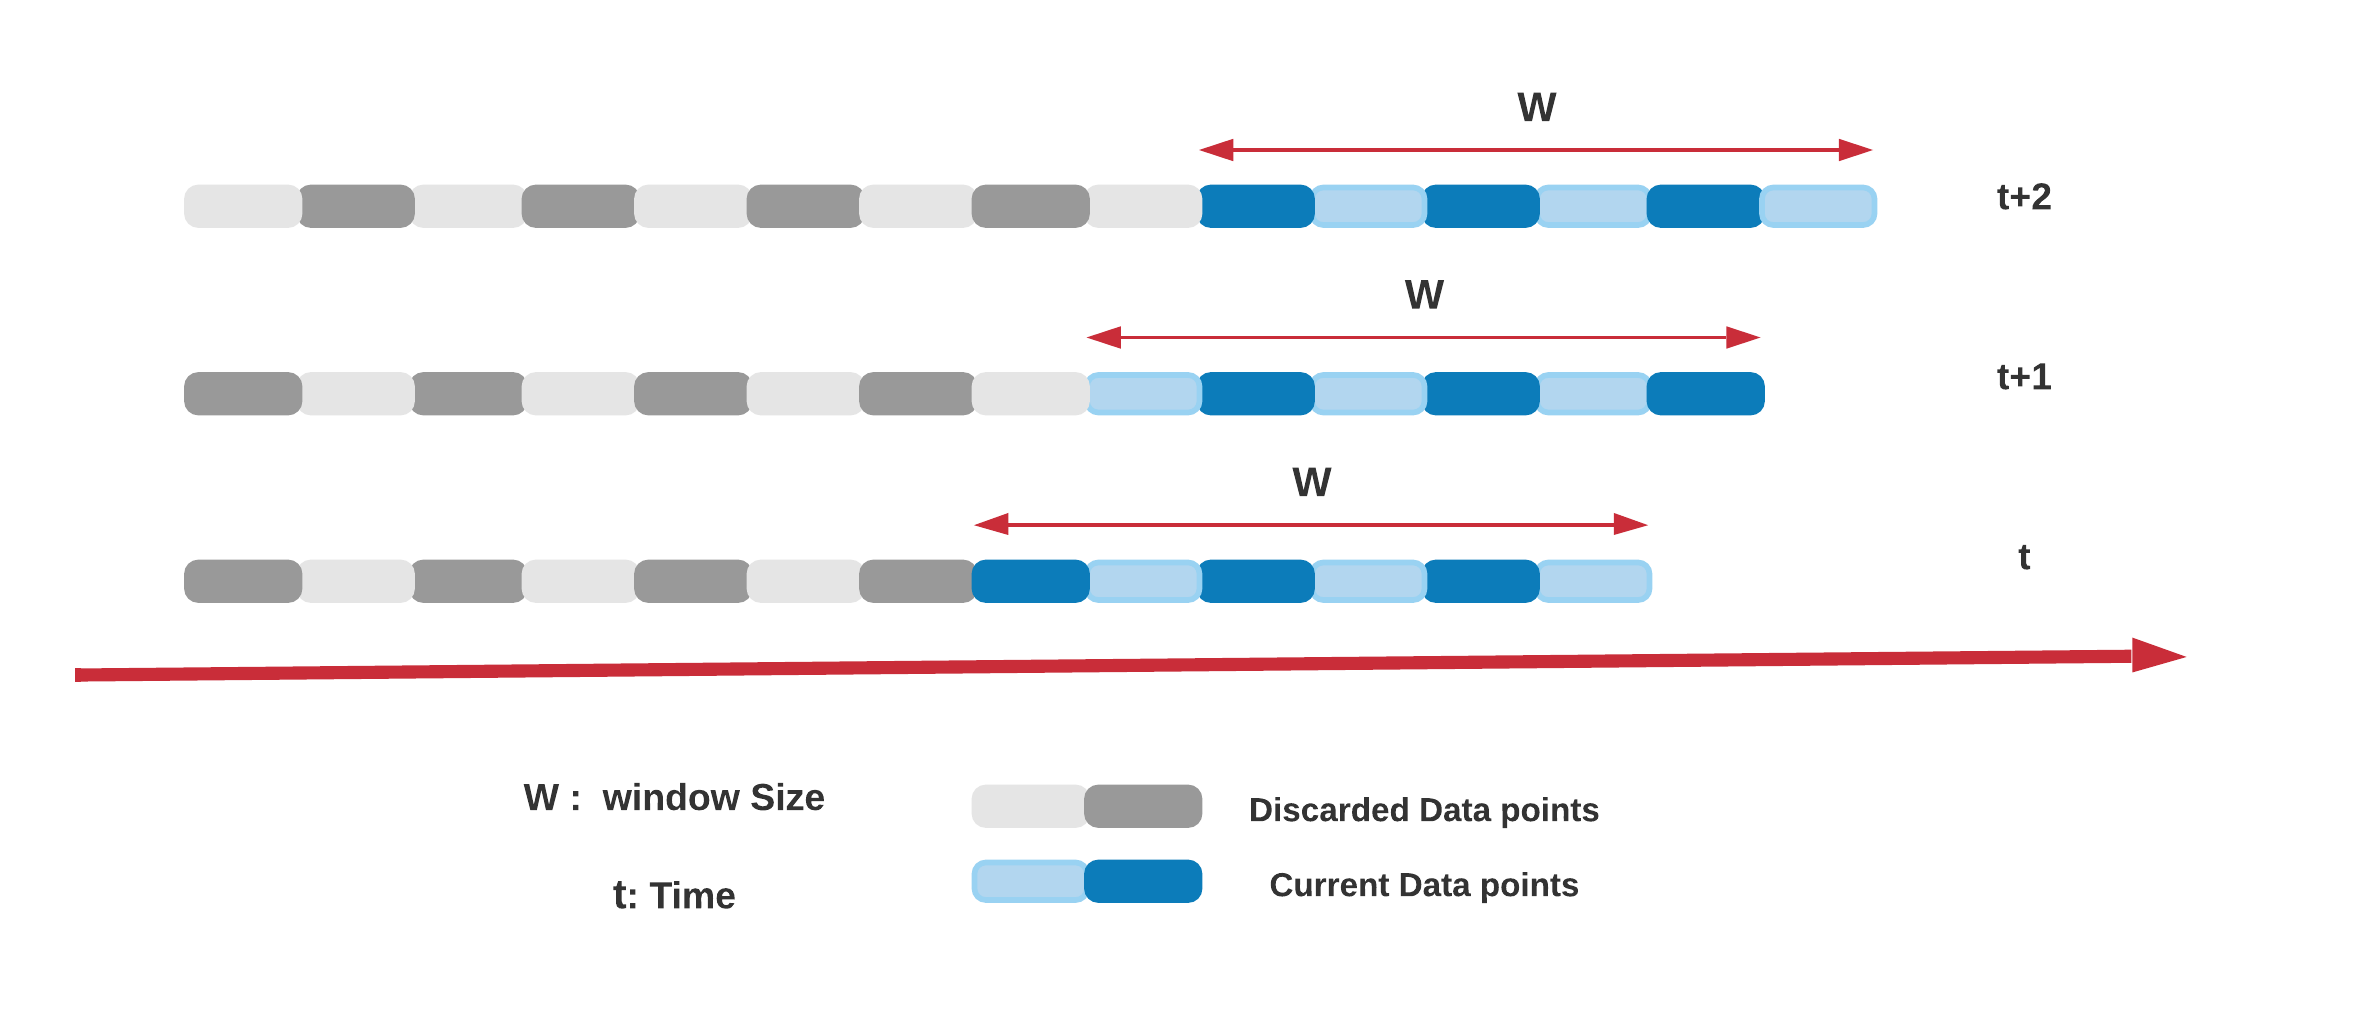
\includegraphics[width = 14cm,height = 7cm]{image/stw (2).png}
% \caption{Sliding time window model applied in this work\cite{zubarouglu2020data}}
% \label{stw}
% \end{figure}
% \cite{zubaroglu2020data}









%%%%%%%%%%%%%%%%%%%%%%%%%%%%%%%%%%%%%%%%%%%%%%%%%%%%%%%%%%%%%%%%%%%%%%%%%%%%%%%%%%

\section{Indoor Localization  and Occupancy Detection}

Location-based services (LBS) become extremely popular and it is part of daily life. The location-based services and their applications require a high level of standard in positioning technology. The positioning technology has shifted from the outdoors to indoor and this is because of two reason \cite{xia2017indoor}. people usually spend most of their time indoors. Besides, most mobile phones and data communications are performed indoors. Moreover, phone data show that the demand for indoor mobile communication is very powerful. 

Indoor localization systems can hire a wide range of technologies such as infrared, RFID, sensors, WiFi, Bluetooth and, etc. Using WiFi is one of the best approach due to availability of mobile device on user side. 

\begin{table}[]
\caption{Comparison between GPS and WiFi technologies.}
\small
\centering
\label{tab:my-table}
\begin{tabular}{@{}ccc@{}}
\toprule
\textbf{Technology} & \textbf{Accuracy level} & \textbf{Advantage}                                                                                    \\ \midrule
GPS                 & High                    & \begin{tabular}[c]{@{}c@{}}*Good accuracy\\ *Not strong for indoor\end{tabular}                       \\ \midrule
WiFi                & Medium                  & \begin{tabular}[c]{@{}c@{}}*Good accuracy for indoor\\ *Limited coverage\\  *Medium cost\end{tabular} \\ \bottomrule
\end{tabular}
\end{table}


The most used method for estimating the location of indoor mobile objects or positioning with WiFi networks is fingerprinting method. The fingerprinting method works based on the signal strength. 






\subsection{Indoor Localization Using Sensors}
The magnificent growth of indoor localization studies can lead to many real-world applications, including smart homes, smart campuses, and localize users to provide services. The purpose of indoor localization is to recognize a location within a multi-storied building with a smart device.  The GPS does not work in an indoor environment accurately as signal strength fluctuates weakly, leading to the user’s device not receiving location updates at fixed periods. 

There are various applications for measuring number of people and occupancy, it can be a simple pen and paper to fully automated, sensor solutions.
Automated solutions use people counting technology to automatically count people as they enter and exit of buildings. People counting is ideal for any kind of buildings that require intelligent system especially for huge and crowded buildings such as malls, hospitals, stadiums, etc. People's movement is precious data for occupancy monitoring, smart building management, and social distancing management.  Using these systems can give users, a better understanding of the workplace and room usage, reduce energy consumption or optimize building design and staff levels.

This technology can be considered in terms of:
\begin{itemize}
    \item\textbf{Accuracy}: Sensors are designed to count number of people at any places continuously.
    \item\textbf{Historical data log}: comprehensive historical data and reports are available with the user requests. Some reports may show how occupancy changes over time, also, how well the building complied with occupancy limits.
    \item\textbf{Cost}: The cost of these sensor may be higher at first for the sensor hardware, however, this is offset by zero or minimal ongoing costs.
\end{itemize}

The bidirectional people counter sensors is one of these types of sensors used for the dataset applied in this research work. The principle of these sensors are based on the interruption of the horizontal infrared beans which usually installed at entrance or exit. However, other technologies such as thermal and stereo-vision can be used. When this infrared bean is interrupted, the receiver detects this movement and it will increase the internal counter. The sensor data will find its way to the server through the gateway SNG. The overview of this scenario shows in Figure \ref{people}. Different types of these sensors are available bellow which they are produced by the International Road Dynamics company  .

\begin{figure}
\centering
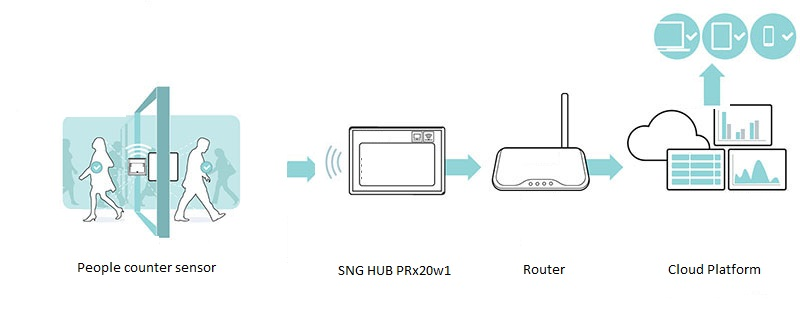
\includegraphics[width = 12cm,height = 5cm]{image/pc.jpg}
\caption{People counter infrastructure used for our experimental dataset. Modified Figure of \protect\cite{SensM}}
\label{people}
\end{figure}


\begin{table}[!h]{}
\small
\centering
\caption{List of people counter sensors of International Road Dynamics company}%\cite{people}.}
\begin{tabular}{llll}
\toprule
\textbf{Features} & \textbf{Transmitter} & \textbf{Receiver}  & \textbf{Applications}     \\
\midrule
Display/Wireless/Bidirectional     &  PTx20-1 & PRx20WD1 & Entrance and daily counts\\ 
Wireless/Bidirectional             &  PTx20-1 & PRx20W1  & Entrance and daily counts\\ 
Display/Bidirectional              &  PTx20-1 & PRx20D1  & Entrance and daily counts\\ 
USB/Bidirectional                  &  PTx20-1 & PRx20U2  & Entrance and daily counts\\ 
Display/USB/Bidirectional          &  PTx20-1 & PRx20UD2 & Entrance and daily counts\\ 
\bottomrule
\label{sensor}
\end{tabular}
\end{table}




\subsection{Indoor Localization Using WiFi}

Automatic user localization calculates the position of the user with knowing latitude, longitude and altitude. This can be calculated by having an electronic device such as a mobile phone. Indoor localization is still a challenging topic and it is because of the loss of GPS signals in indoor environments.

Wireless-based indoor localization is another way for measurements. Wireless waves can go through obstacles like walls or doors and provide ubiquitous coverage of a building. WLAN indoor localization uses received signals value (RSSI) to indicate the distance to points and get the current point's location.
This architecture need two things, the beacon station that emits the wireless signals and electronic devices such as cellphones. 
Fingerprint means the characteristic or feature of signals which RSS can be one of them. The assumption underneath this fingerprint-based indoor localization is that for each position in the area, the signals' features are different. By relying on the variation of signals in a distinct position, the current location can be obtained.



% \begin{figure}
% \centering
% 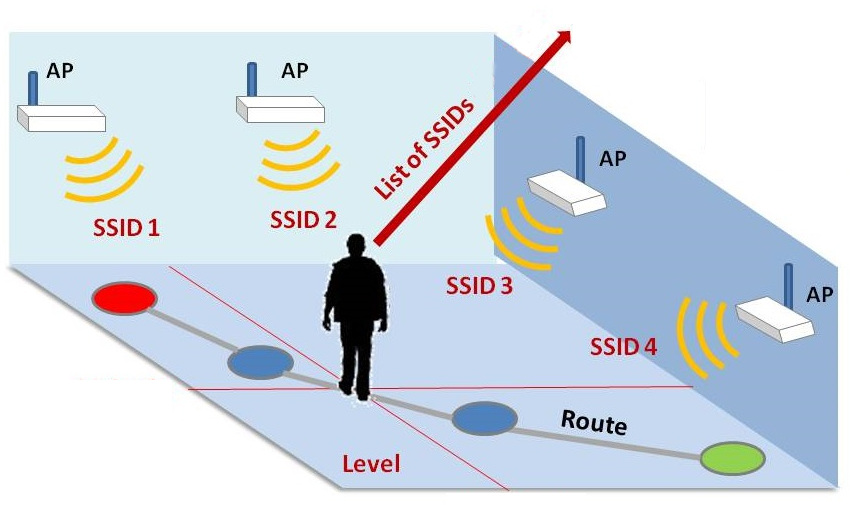
\includegraphics[width = 9cm,height = 6cm]{image/indoorp.jpg}
% \caption{Indoor positioning technique using WLAN . }
% \label{time}
% \end{figure}

%elmi


%elmi. RSSI, or “Received Signal Strength Indicator,” is a measurement of how well your device can hear a signal from an access point or router.  RSSI is a term used to measure the relative quality of a received signal to a client device, but has no absolute value. The IEEE 802.11 standard (a big book of documentation for manufacturing WiFi equipment) specifies that RSSI can be on a scale of 0 to up to 255 and that each chipset manufacturer can define their own “RSSI Max” value. Cisco, for example, uses a 0-100 scale, while Atheros uses 0-60. Since RSSI varies greatly between chipset manufacturers,

%elmi. wiki.In an IEEE 802.11 system, RSSI is the relative received signal strength in a wireless environment, in arbitrary units. RSSI is an indication of the power level being received by the receiving radio after the antenna and possible cable loss. Therefore, the greater the RSSI value, the stronger the signal. Thus, when an RSSI value is represented in a negative form (e.g. −100), the closer the value is to 0, the stronger the received signal has been. There is no standardized relationship of any particular physical parameter to the RSSI reading. The 802.11 standard does not define any relationship between RSSI value and power level in milliwatts or decibels referenced to one milliwatt (dBm). Vendors and chipset makers provide their own accuracy, granularity, and range for the actual power (measured as milliwatts or decibels) and their range of RSSI values (from 0 to RSSI maximum).[2] One subtlety of the 802.11 RSSI metric comes from how it is sampled—RSSI is acquired during only the preamble stage of receiving an 802.11 frame, not over the full frame.[3]

%Elmi. The wifi ujindoorloc can be used as an example wlan suvey data to determine the signal coverage and the density of people could be used for capacity estimation. Cisco wlan deployment guideline.




%%%%%%%%%%%%%%%%%%%%%%%%%%%%%%%%%%%%%%%%%%%%%%%%%%%%%%%%%%%%%%%%%%%%%%%%%%%%%%%%%%%%%%%%%%%%%%%






%{Scalability of Clustering Methods}
%Handling large-scale and dealing with real datasets is a key concern. High performance and large memory size cannot give accurate clustering. This section explain methods to keep the clustering computational beyond these limits.


%\subsection{Time window models for clustering}
%%---------------time window-----------------------------------------------




% \section{Positioning Technologies and Application Fields for Clustering/Spatiotemporal data clustering}

%positioning technologies
%Ecounter and Wifi examples of data.
%how ecounters work
%how wifi localization data works





% \subsection{Indoor People Counting }


% \subsection{Automatic user localization: Wi-Fi positioning system}







% \begin{table}[ht]
%     \centering
%     \caption{comparison between K-means and AP }
%     \label{comp}
%     \begin{tabular}{|c|c|c|}
%     \hline
%       & K-means & AP \\
%      \hline
%      exemplar &  generate  & actual point\\
%      \hline
%      parameters & $K$  & $S^*(penalty)$\\
%      \hline
%      algorithm & greedy search  & message passing\\
%      \hline
%     performance &  not stable & stable\\
%      \hline
%       complexity & $N * K$   & $N^2 log(N)$\\
%       \hline
     
%     \end{tabular}
    
% \end{table}


  
\end{document}


%\subsection{Sliding Time Window for the Workflow}
%**********elmi
%To enable processing of blocking operators like average and sum over infinite data streams, windowing is commonly used in data stream processing because it limits the extent of data to a sequence of most recent elements in the data stream. Clustering algorithms are blocking since they require having all the data points to compute the clusters. Therefore, windowing is needed for data stream clustering.There are different ways of defining a window over a data stream \cite{xu2016scalable}.The window specification defines how recent stream elements are selected for windowing. When the window specification is applied on a live data stream it produces new window instances at different points in time. A window instance logically contains a set of stream elements.For example, a sliding window is specified by defining its range and stride. The range R of a sliding window specifies the length of the window while the stride S specifies the portion of the range that is evicted from the window when the window moves forward. A sliding window is specified as a tuple <R,S>, where S<R. Two common kinds of sliding windows are time-based and count-based sliding windows \cite{li2014parallel}. In time-based sliding windows R and S are defined using time intervals while in count-based sliding windows they are defined in terms of the number of elements. For example a time based sliding window with R=10min and S=2min produces window instances that cover the data in the last 10 minutes of the stream and a new window instance is created every 2 minutes. Without loss of generality, we present sliding windows using count-based sliding windows. %**********


%Generally, a clustering method for data stream is originated from a corresponding clustering method for batch data, e.g., CluStream from K-means, DenStream from DBSCAN, and STRAP from AP clustering. THIS BELONGS TO LR

%Data stream clustering finds clusters based on the flow of data, and it is different from traditional clustering \cite{toshniwal2013clustering}:

%\begin{itemize}
    % \item Traditional clustering data are static; the data stream is dynamic.
    % \item Traditional clustering datasets can be accumulated in memory, but the streaming data is enormous in size, and then it is not possible to store in memory.
    % \item traditional clustering results are fixed, but The data stream clustering results vary over time.
%\end{itemize}




%
% \begin{enumerate}
%     \item\textbf{Data collection phase:} The data collection phase involves gathering observations or measurements from sensors, cameras, or electronic devices.
    
%     \item\textbf{Data prepossessing phase:}  Real-world data is sometimes incomplete, inconsistent, and contains errors. Various techniques have evolved for handling and transforming the data into a usable format. This phase consists of data cleaning, data transformation, and aggregation stages.
    
%     \item\textbf{Data Stream Simulation Phase:} Convert the batch of data to the stream fashion. 
    
%     \item\textbf{Data Stream Clustering Phase:}Generates micro and macro clusters using a sliding time window. 
    
%     \item\textbf{Clustering Performance Evaluation Phase:} Computing cluster measurements to evaluate the quality of the clusters by the target Coefficient and indexes.
% \end{enumerate}






% \section{Data Stream Simulation}
% Since data used in this research were obtained from concluded experiments, it was essential to find a mechanism to convert the batches of data in to a data stream. The streaming data was generated from the target datasets by applying the Scikit-Multiflow package in Python for the DSAP algorithm and the DSD objects in the stream package in R for the streaming K-means algorithm. 



% \subsection{Scikit-Multiflow-based Simulation}
% The 'scikit-multiflow' framework in Python programming language is a free and open-source tool for generating data stream \cite{montiel2018scikit}. It provides multiple stream learning methods, steam generators, and evaluators, where the primary focus is on batch learning. This framework's base class is the 'StreamModel', which has abstract methods to be implemented by classes. A 'StreamModel' object interacts with other objects: ' Stream' and 'StreamEvaluator'. The 'stream' gives an endless flow of data by request, and 'StreamEvaluator' presents various tasks that are queries the stream, train, test on the incoming data, and tracks the model's performance.

% 'scikit-multiflow' needs NumPy library installed in the system. All classes are shown in Figure \ref{sci} for generating data stream. The \textit{skmultiflow} data contains data stream methods, including methods for batch-to-stream conversion and generators. In all classes, the stream is available upon request and old data points cannot be accessed at a later time. These are listed below:

% %\renewcommand\labelitemi{$\vcenter{\hbox{\tiny$\bullet$}}$}
% \begin{itemize}
%     \item {data.base\_stream.Stream:} it defines the minimum requirements of a stream and it can work along with other modules in multiflow. 
%     \item {data.DataStream:} it takes the whole data consisting of the $X$ as features and $Y$ as targets or takes them separately.
%     \item {data.FileStream:} if the data previously collected and stored in the CSV file (it just supports CSV files at this moment), it can generate streams by loading the dataset. 
%     \item {data.ConceptDriftStream:} this stream generator adds concept drift by joining several streams and giving the weight. 
%     \item {data.TemporalDataStream:} takes the dataset containing $X$ as a features and $Y$ as a targets with $time$ as a timestamps. 
% \end{itemize}

% On the other hands, as shown in Figure \ref{sci}, there are many stream generators classes for different problems listed below:
% %\renewcommand\labelitemi{$\vcenter{\hbox{\tiny$\bullet$}}$}

% \begin{itemize}
%     \item[$-$]  data.WaveformGenerator: random differentiation of some base waveforms.
%     \item[$-$]  data.SineGenerator: sine waves stream generator.
%     \item[$-$]  data.AgrawalGenerator: scaling up decision tree learners based on Agrawal model.
%     \item[$-$]  data.AnomalySineGenerator: simulate a stream with anomalies in sine waves.
%     \item[$-$]  data.LEDGenerator: seven-segment LED display stream generator.
%     \item[$-$]  data.LEDGeneratorDrift: add concept drift to the LED stream.
%     \item[$-$]  data.MixedGenerator:  data stream with abrupt concept drift and boolean noise-free.
%     \item[$-$]  data.MultilabelGenerator: the stream of samples for a multi-label problem.
%     \item[$-$]  data.RandomRBFGenerator: Random Radial Basis Function stream generator.
%     \item[$-$]  data.RandomTreeGenerator: based on a random tree that splits features at random and sets. 
%     \item[$-$]  data.RegressionGenerator: creates a regression stream.
% \end{itemize}


% \begin{figure}
% \centering
% 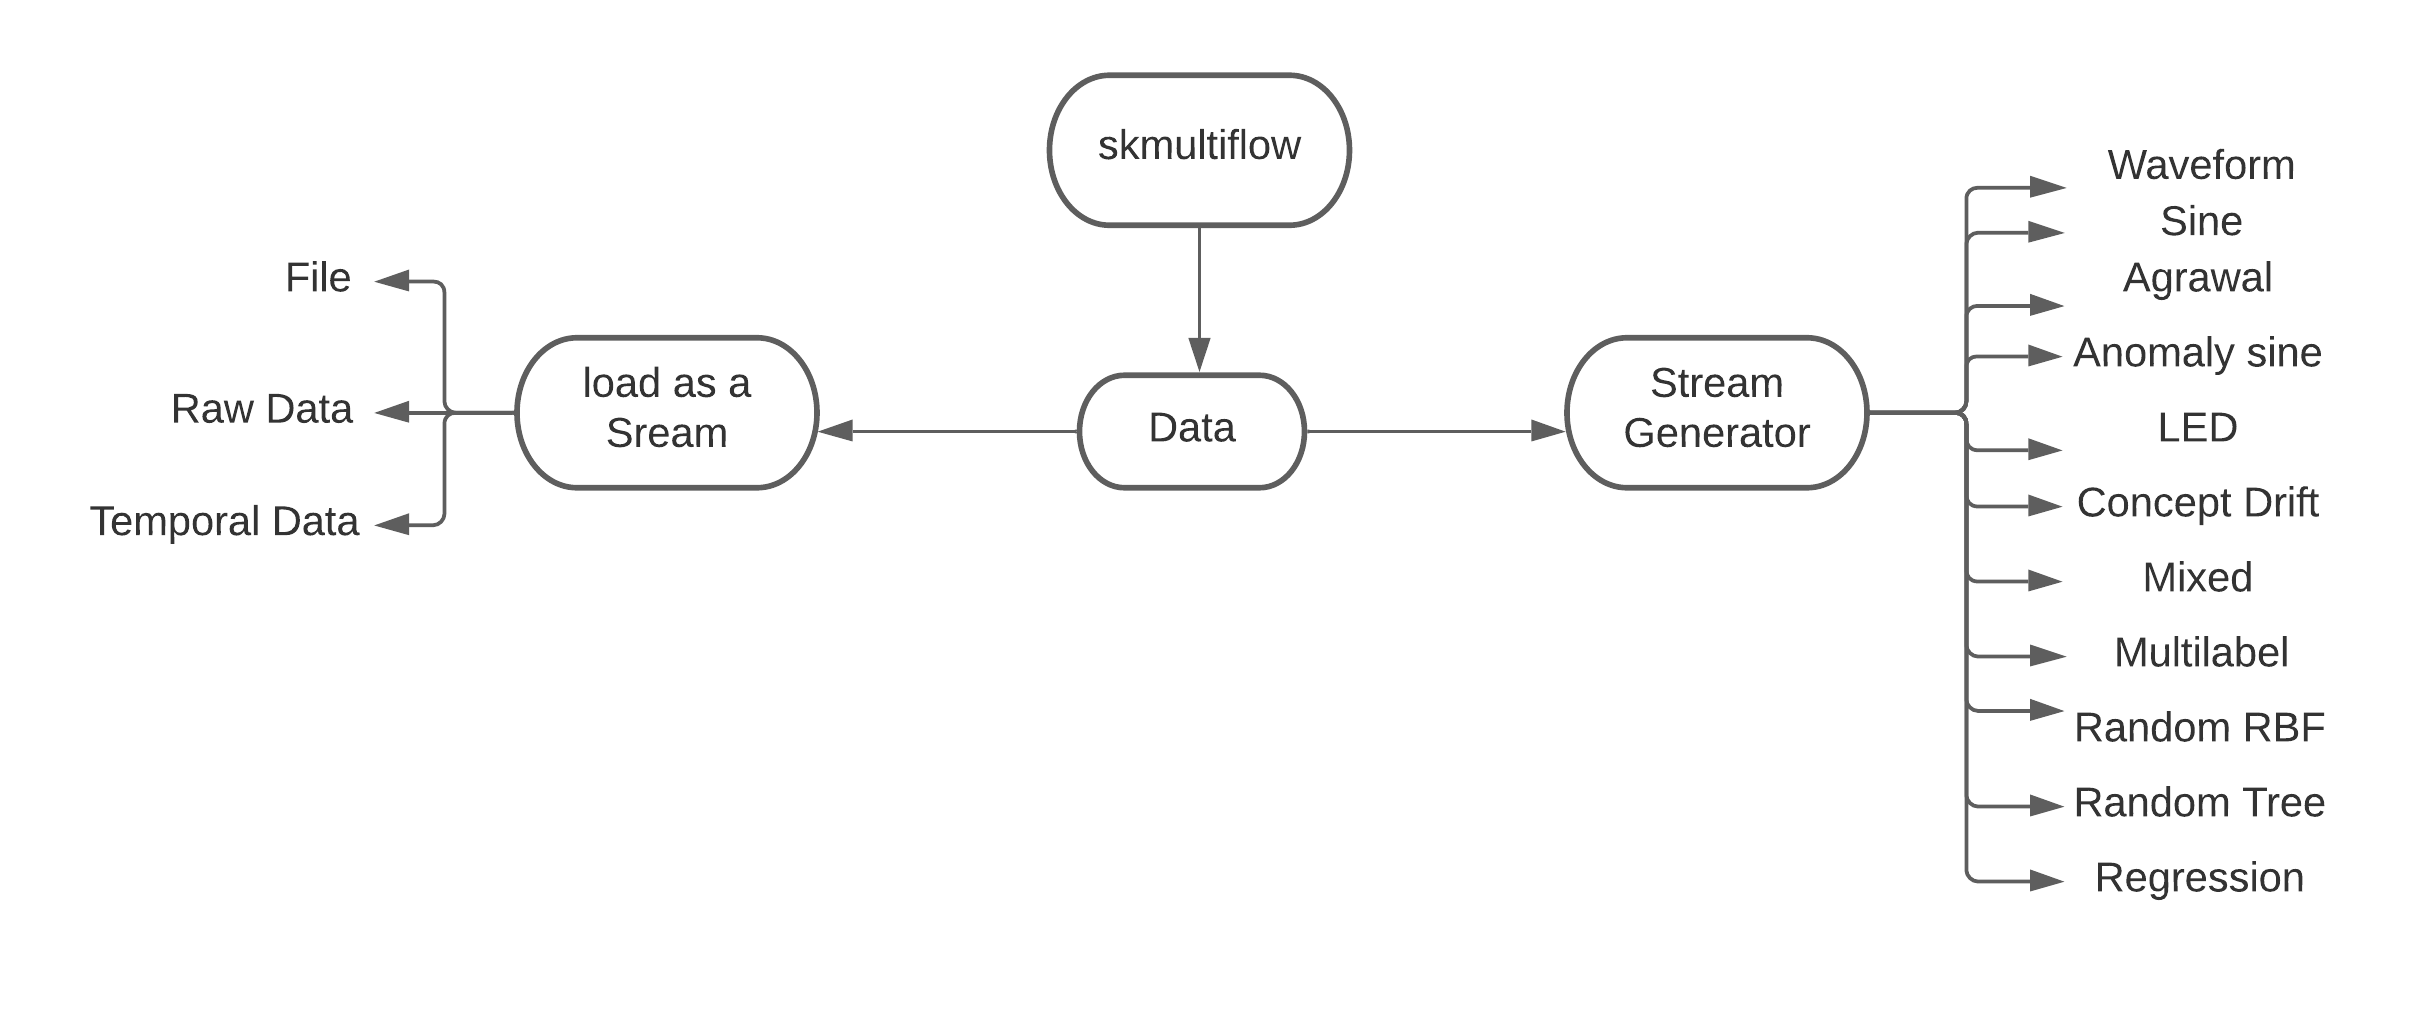
\includegraphics[width = 12cm,height = 6cm]{image/sci2.png}
% \caption{The scikit-multiflow map with multiple methods for generating data. }
% %\cite{SMF}}
% \label{sci}
% \end{figure}



% The k-means algorithm can be explained by the following 4 steps:
% Step 1: define the number of clusters (K) and randomly pick k instances as the initial cluster centroids.
% Step 2: assign all data points to the closest centroid by measuring the distance such as the Euclidean distance.

% Step 3: re-compute the centroid of each cluster by calculating mean value of all the data points in the cluster.
% Step 4: repeat steps 2 and 3 until the centroid does not change.
% https://pdfs.semanticscholar.org/1040/6a6e1319a48e731db73ed22bbde61fa42691.pdf


% \section{Comparison  Between  DSAP  and  Streaming  K-means Phase}
% The general approach of the various stream clustering algorithms that allow for the investigation of the cluster structure at different time intervals are fairly similar. They typically have two stages, online where the algorithm maintain a summary of the data as micro-clusters and next in the offline phase the summary micro-clusters are clustered to provide real insights to the data. The efficiency of these algorithms are greatly affected by the choice of the clustering algorithm used. We have introduced the DSAP algorithm for data stream clustering which is implemented based on the AP algorithm. This model is compared with the established streaming K-means algorithm introduced earlier in Chapter 2. It is known that the AP algorithm usually generates results that show that the k-means algorithm is faster than AP. However, streaming AP based algorithms has been shown to provide similar quality clusters as k-means based ones but, the results tend to be more robust.

% K-means algorithm is scalable for large datasets with different shapes and sizes and is easy to implement. The K-means algorithm is known to easily adopt to new centroids and is one of the fastest algorithms out there owing to a linear time complexity. Also, K-means guarantees convergence by trying to minimize the total sum of the square error as an objective function over the number of iterations. On the other hand, the K-means algorithm has some known drawbacks. Finding the $k$ optimum number of clusters is not a precise task that can be accurately automated. The algorithm results are a function of the initial clusters chosen and necessitate multiple runs of the algorithm with the different values to pick the most suitable clusters. During data stream clustering this process can be time consuming and make the model less accurate. The algorithm is known to have difficulties in finding the right clusters for data with varying size and density. In addition, K-means clusters centroids are affected by outliers since the mean as a statistic is sensitive to outliers. %it means outliers can drag the centroids or they may have their own centroids. 
% Lastly, even though K-means can be easily scaled to large datasets but it has difficulties to cluster high-dimension data. 


% In comparison with the K-means algorithm that needs to determine the optimal number of clusters prior by applying some methods like elbow method, the AP algorithm calculates the number of clusters internally. However, AP needs additional parameters like the damping factor and preference to be set since the model convergence is dependent on the damping parameter while the preference controls the probability of finding centroids. Due to the additional complexities in the calculation of AP it becomes prohibitively expensive to scale AP as compared to the K-means which scales linearly with the size of the dataset. The semi-supervised selection of the number of clusters in K-means limits the potential of producing large number of clusters that can sometimes be generated by the AP if it's parameters are not chosen carefully. Both these partitioning based algorithms can be evaluated based on metrics that quantify the density and spread of the clusters. 

% Affinity propagation has been shown to perform well in pattern recognition applications in the fields of computer vision and computational biology. The main advantage of AP is the robustness of its optimization. While K-means follows a greedy optimization method to find the optimum of the optimization problem, AP tackles a continues optimization problem, in which all data points are potential candidate at the beginning and clusters are gradually identified. AP does not suffer from the initialization can guarantee global optimization consistently.


